%\documentclass[11pt,a4paper,twoside]{tesis}
% SI NO PENSAS IMPRIMIRLO EN FORMATO LIBRO PODES USAR
\documentclass[11pt,a4paper]{tesis}

\usepackage{graphicx}
\usepackage[utf8]{inputenc}
\usepackage[spanish]{babel}
\usepackage[left=3cm,right=3cm,bottom=3.5cm,top=3.5cm]{geometry}

\usepackage{color}
\usepackage{solucion}
\usepackage{multicol}
\usepackage{float}
\usepackage[linesnumbered,ruled,lined,spanish]{algorithm2e}
\usepackage{xcolor}
\usepackage{colortbl}
\usepackage{lscape}
\usepackage{longtable}
\usepackage{amsmath}
\usepackage{amssymb}
\usepackage{textcomp}
\usepackage{caption}
\usepackage{subcaption}
\usepackage{hyperref}
\usepackage{todonotes}
\hypersetup{
    colorlinks,
    citecolor=black,
    filecolor=black,
    linkcolor=black,
    urlcolor=black
}
\usepackage[many]{tcolorbox}

\newtcolorbox{mybox}[1]{
    tikznode boxed title,
    enhanced,
    arc=0mm,
    interior style={white},
    attach boxed title to top center= {yshift=-\tcboxedtitleheight/2},
    fonttitle=\bfseries,
    colbacktitle=white,coltitle=black,
    boxed title style={size=normal,colframe=white,boxrule=0pt},
    title={#1}
}

\DeclareMathOperator*{\argmin}{arg\,min}
\DeclareMathOperator*{\argmax}{arg\,max}
\begin{document}

%%%% CARATULA
% Comentar y descomentar según corresponda
\def\titulo{Licenciado }
\def\autor{Amit Stein, Juan Andrés Knebel}
\def\tituloTesis{Nuevos algoritmos para recuperación de ``ítems empaquetados'': \mbox{Algo}}
\def\runtitulo{Nuevos algoritmos para recuperación de ``ítems empaquetados''}
\def\runtitle{New Algorithms for composite retrival}
\def\director{Obi-Wan Kenobi}
\def\codirector{Master Yoda}
\def\lugar{Buenos Aires, 2016}
%\newcommand{\HRule}{\rule{\linewidth}{0.2mm}}
%
\thispagestyle{empty}

\begin{center}\leavevmode

\vspace{-2cm}

\begin{tabular}{l}

\includegraphics[width=2.6cm]{logofcen.pdf}
\end{tabular}


{\large \sc Universidad de Buenos Aires

Facultad de Ciencias Exactas y Naturales

Departamento de Computaci\'on}

\vspace{6.0cm}

%\vspace{3.0cm}
%{
%\Large \color{red}
%\begin{tabular}{|p{2cm}cp{2cm}|}
%\hline
%& Pre-Final Version: \today &\\
%\hline
%\end{tabular}
%}
%\vspace{2.5cm}

{\huge\bf \tituloTesis}

\vspace{2cm}

{\large Tesis presentada para optar al t\'{\i}tulo de\\
\titulo en Ciencias de la Computaci\'on}

\vspace{2cm}

{\Large \autor}

\end{center}

\vfill

{\large

{Director: \director}

\vspace{.2cm}

{Codirector: \codirector}

{Codirector: \codirectordos}

\vspace{.2cm}

\lugar
}

\newpage\thispagestyle{empty}


%%%% ABSTRACTS, AGRADECIMIENTOS Y DEDICATORIA
\frontmatter
\pagestyle{empty}
%\begin{center}
%\large \bf \runtitulo
%\end{center}
%\vspace{1cm}
\chapter*{\runtitulo}

\noindent Las búsquedas tradicionales nos ofrecen una solución que solo tiene en cuenta un atributo de los elementos y no la relación que éstos tienen con el resto del universo. Las mismas nos ofrecen un lista ordenada de resultados que cumplen con el criterio elegido en mayor o menos medida, ocasionando que muchas veces se necesite reformular la consulta original para así lograr la solución que el usuario quiere encontrar.\\
Los algoritmos de agrupación clásicos o clustering generan conjuntos de soluciones, que al igual que las búsquedas tradicionales, los elementos dentro de cada conjunto o cluster cumplen con el criterio elegido y además entre sí comparten alguna propiedad (generalmente una similitud o distancia), pero no se analiza ningún tipo de Complementaridad entre los elementos. La relación entre los cluster no es analizada ocacionando que entre ellos sean muy similares o diferentes dependiendo del universo en el cuál se encuentre trabajando.\\
Es por eso que surge \textbf{Composite Retrieval}, su objetivo es agrupar elementos en cluster bajo un mismo atributo, al mismo tiempo que éstos son complementarios entre sí por algún atributo definido previamente. A diferencia de las anteriores técnicas se permite elegir el grado de interdepencia entre los conjuntos generados permitiendo, según el caso, que los conjuntos que componen la solución sean más o menos parecidos facilitando al usuario la elección de un grupo de elementos que satisfagan su consulta original.

\bigskip

\noindent\textbf{Palabras claves:} Composite Retrieval, Similitud, Complementaridad, Búsqueda Tabú, Generación de Bundles, Agrupamiento.

\cleardoublepage
%%\begin{center}
%\large \bf \runtitulo
%\end{center}
%\vspace{1cm}
\chapter*{\runtitulo}

\noindent Las búsquedas tradicionales ofrecen soluciones que solo tienen en cuenta un solo atributo de los elementos y no la relación que estos tienen con el resto del universo. Las mismas suelen ofrecer una lista ordenada de resultados relacionadas con
el criterio utilizado. Ocasionando, muchas veces, re formular la consulta original para así lograr una solución adecuada al criterio de búsqueda elegido previamente.\\
Los algoritmos de agrupación clásicos o clustering generan conjuntos de soluciones, al igual que las búsquedas tradicionales, en los cuales los elementos dentro de cada conjunto (o cluster) tiene una relación directa con la búsqueda original y además se encuentran relacionados de alguna manera (generalmente una similitud o distancia). Aún así, éstas soluciones no tienen en cuenta ningún atributo que represente la complementaridad que existe entre los elementos, ocasionando que la solución encontrada contenga conjuntos de objetos muy similares sin diversidad. La relación entre los cluster no es sujeto de ningún análisis en estos algoritmos. En orden de lograr una solución con mayor diversidad (evitar cluster similares) y que cumpla las expectativas del usuario, debería existir un análisis entre los clusters.\\
Como respuesta a éste último comportamiento surge Composite Retrieval of Diverse and Complementary Bundles \cite{compositeRetrival}, su objetivo es agrupar elementos en bundles en los cuales los elementos dentro de ellos se encuentran relacionados internamente bajo algún criterio de similitud y a la vez sean complementarios de forma tal que satisfaga las expectativas del usuario y no tenga la necesidad de realizar una nueva intervención logrando así una mejor experiencia de búsqueda.\\
En este trabajo se tomaron las ideas ya desarrolladas previamente en \cite{compositeRetrival}, se propuso un nuevo algoritmo, nuevas mejoras y enfoques en orden de mejorar los resultados que se obtuvieron originalmente y los tiempos de ejecución para instancias más grandes. Las nuevas aplicaciones se aplicaron a la resolución de búsquedas sobre una base de datos de artículos científicos pertenecientes a la Ingeniería de Software \cite{dataDrive} y sobre una instancia conformada por atracciones turísticas de Europa.

\bigskip

\noindent\textbf{Palabras claves:} Composite Retrieval, Similitud, Complementaridad, Búsqueda Tabú, Generación de paquetes, Agrupamiento.

%\cleardoublepage
%\chapter*{Agradecimientos}

\noindent A Laura que estuvo a mi lado
\noindent A mis padres, a Abigail y René y a Edith que me acompañaron y ayudaron durante toda la carrera y A Mila y Florián que lo hicieron este último tramo. 
\noindent a todos los profesores y ayudantes del DC y en especial a Paula, Isabel y Estebán por todo lo enseñado.
\noindent A Dario, Julio y Sebastián con los que además de compañeros nos hicimos buenos amigos.
\noindent A Anita que me acompañó y me apoyó en todos estos últimos años de mi vida y que hace que cada día sea más lindo que otro.
\noindent A todo mi familia por todo lo que me dieron sin pedir nada: Hugo, Graciela, Nicolas, Luciana, Marco, Blas, Julia, Carlita.
\noindent A mis amigos de siempre de Bahía Blanca por bancarme en todas.
\noindent A Ezequiel Cura que aunque solo cursamos una sola vez y no veamos poco, es un gran amigo.
\noindent A mis compañeros de trabajo de Technisys que se aguantaron tantas charlas de este trabajo. % OPCIONAL: comentar si no se quiere

%\cleardoublepage
%\hfill \textit{A Nestor y Chavez que nos cuidan y guian desde arriba}  % OPCIONAL: comentar si no se quiere

\cleardoublepage
\tableofcontents

\mainmatter
\pagestyle{headings}

%%%% ACA VA EL CONTENIDO DE LA TESIS

\chapter{Introducción}
\label{chap:introduccion}
\section{Estado Actual de las Búsquedas}
{\begin{small}%
\begin{flushright}%
\it An algorithm must be seen to be believed.\\Donald Knuth.
\end{flushright}%
\end{small}%
\vspace{.5cm}}
Las búsquedas son acciones que se llevan a cabo con el fin de hallar elementos. Para lograr el objetivo el usuario debe ingresar frases o términos relacionados a fin de encontrar los resultados deseados. A lo largo del desarrollo de Internet las búsquedas fueron adquiriendo cada vez más importancia por la enorme cantidad de información que cada día se almacena en los distintos servidores a lo largo del planeta.\\
En un principio los algoritmos utilizados eran más simples o se basaban únicamente en buscar coincidencias exactas de las frases ingresadas en los elementos a buscar. Con el paso del tiempo las estrategias fueron evolucionando y adaptándose, con el objetivo de devolverle al usuario resultados más completos y que a la vez sean relevantes.\\
La \textbf{Recuperación de la Información} (IR por Information Retrieval en inglés), es la actividad de obtener información relevante de una inmensa colección de datos y con criterios de lo más variados, desde el resultado de la final del mundial de fútbol, los libros de un autor y hasta el mail de la confirmación de una compra.\\
Los motores de búsquedas de la web como Google, Yahoo y otros, son los clásicos ejemplos de una aplicación de IR. El proceso de búsqueda comienza cuando el usuario ingresa una consulta de la que el buscador devuelve una colección de elementos que coinciden con el criterio de búsqueda. En general lo que ocurre es que son varios los elementos del universo que concuerdan pero con grados de relevancia diferentes (ranking de resultados) que se utiliza para ordenar la colección de elementos devueltos. Para obtener el ranking de resultados los sistemas de IR trabajan con una representación lógica de los elementos que incluye los metadatos necesarios para operar sobre ellos. La desventaja de los ranking de resultados es que únicamente se compara la consulta de la búsqueda con los metadatos de los elementos, dejando de lado el análisis de los elementos entre sí y conviritiendo, en ocasiones, al proceso en una acción tediosa y repetitiva ya que el usuario deberá cambiar la consulta original y explorar la colección de elementos hasta lograr encontrar el o los elementos deseado.\\
En el  artículo \textbf{Composite Retrieval of Diverse and Complementary Bundles}\cite{compositeRetrival} se propone presentar una lista de grupos de elementos, en lugar de entregar una lista vertical de los mismos. Cada grupo deberá estar relacionado internamente bajo el criterio de similitud elegido y la lista ordenada de forma lógica con la finalidad de que uno o más conjuntos satisfagan las expectativas del usuario sin necesidad de una nueva intervención para refinar su búsqueda para lograr una mejor experiencia de búsqueda.\\
La finalidad de este trabajo es devolver los resultados de las búsquedas como plantea el artículo \textbf{Composite Retrieval of Diverse and Complementary Bundles} para ello se analizaron e implementaron los algoritmos de agrupamiento (o clustering) que realizan la tarea de agrupar en conjuntos disjuntos a elementos que pertenecen a una misma clase. Las dos técnicas más usadas son agrupamiento jerárquico y no jerárquico. La primera a su vez se puede dividir en dos tipos, aglomerativos donde todos los elementos comienzan como un cluster para luego mezclarse entre ellos y divisivos en el cual se comienza con un único grupo y se comienza a dividir. Para las decisiones de unir o dividir se usan medidas de similitud o disimilitud de los elementos del conjunto. Para la segunda técnica de clusterización se definen previamente cuales serán los grupos finales y se van asignado los demás elementos al grupo que correspondan. Además de las técnicas de clusterización, se desarrollaron heurísticas para buscar una solución mejor.\\
\section{Motivación}
Planear un viaje típicamente requiere realizar múltiples búsquedas en distintos motores para recabar la información de los diferentes destinos que se quiere visitar, las distancias geográficas, los precios de las atracción o leer opiniones acerca de los destinos seleccionados, entre otros.\\
En una búsqueda típica los resultados obtenidos son una larga lista ordenada por la relevancia del criterio de la consulta. Este tipo de soluciones no otorgan respuestas que relacionen el criterio buscado con los demás elementos de la lista resultante.\\
Otro ejemplo es el caso en el que un cliente de una tienda online de venta de discos que le gusta escuchar música de diferentes países, cuenta con un presupuesto limitado y no está interesado en un ningún género musical específico, pero si quiere comprar un conjunto de discos que pertenezcan al mismo género musical. El cliente al comenzar su búsqueda obtendría una lista parecida a la siguiente:
\begin{itemize}
  \item Physical Graffiti - Led Zeppelin
  \item Led Zeppelin - Led Zeppelin
  \item It's Hard - The Who
  \item Perfect Strangers - Deep Purple
  \item El Cielo Puede Esperar - Attaque 77
  \item Wheels of Fire - Cream
  \item Confesiones de Invierno - Sui Generis
  \item The White Album - The Beatles
  \item Innuendo - Queen
  \item Sticky Fingers - The Rolling Stones
  \item Kamikaze - Luis Alberto Spinetta
\end{itemize}

De la lista obtenida el usuario deberá seleccionar aquellos discos que sean de su interes con el posible error de elegir más de un disco del mismo origen. Segundo, deberá ir agregando y eliminando de su lista manualmente en el caso que la elección de un disco superase el presupuesto que él posee. Tercero, no necesariamente elegirá el mejor subconjunto de discos que maximice su presupuesto y a su vez el origen de los discos sean distintos.\\
Para este tipo de búsquedas la solución que se propone está pensada para aquellas consultas que requieren obtener un conjunto de elementos que se relacionan como respuesta. Se podría realizar una clusterización de los resultados pero, en las técnicas tradicionales la agrupación se hace por la similitud entre ítems. En el ejemplo de los discos con una clusterización tradicional, donde la similitud sea el género musical, seguramente se generen tantos cluster como géneros de discos existan y en cada cluster se encontrarán todos los discos de ese género. Una vez obtenido el resultado se deberá explorar todos los clusters para elegir los discos.\\
En cambio si se aplicase las técnicas mencionadas en \textit{``Composite Retrieval of Diverse and Complementary Bundles''} las soluciones obtenidas se ajustarían al presupuesto y cada uno de los ítems dentro del bundle (es el nombre que se le da al agrupamiento de ítems) sean complementarios entre sí, de modo tal, que el usuario pordrá optar por cualquier bundle de la solución y estar seguro que su elección cumple con su objetivo inicial, que pertenece a un mismo género musical y exista variedad en la elección.\\
Si en el ejemplo de la tienda de discos se establece la complementariedad del atributo que refleja el origen de la banda y se establece un presupuesto máximo a cada bundle, una solución posible sería:
\begin{itemize}
  \item Bundle 1:
  \begin{itemize}
    \item Physical Graffiti - Led Zeppelin (Inglaterra)
    \item After chabón - Sumo (Argentina)
    \item Back in Black - AC/DC (Estados Unidos)
  \end{itemize}
  \item Bundle 2:
  \begin{itemize}
    \item Natty Dread - Bob Marley (Jamaica)
    \item El ritual de la Banana - Los Pericos (Argentina)
    \item Labour of Love - UB40 (Inglaterra)
  \end{itemize}
	  \item Bundle 3:
  \begin{itemize}
    \item Ramones - Ramones (Estados Unidos)
    \item El Cielo Puede Esperar - Attaque 77 (Argentina)
    \item Sandinista! - The Clash (Inglaterra)
  \end{itemize}
\end{itemize}
Lo que se quiere lograr en los ejemplos descriptos y en cualquier otro problema similar de búsquedas es otorgarle al usuario un conjunto de bundles que cumplan siempre con las siguientes propiedades: 
\begin{itemize}
  \item \textbf{Cubrimiento}: Maximizar la cantidad de elementos en el bundle.
  \item \textbf{Compatibilidad}: Los elementos del bundle deben ser similares.
  \item \textbf{Validez}: El costo total de los elementos del bundle no debe superar el presupuesto.
  \item \textbf{Diversificada}: Los bundles entre si deben ser diversos.
\end{itemize}

\chapter{Trabajos previos}
\label{chap:trabajos-previos}
En la literatura se pueden encontrar trabajos que abordan la noción de recuperación de información con diferentes semánticas. Por ejemplo, en \cite{BasuRoy:2010:CEC:1807167.1807258} se plantea devolver información complementaria de un ``ítem central'' (\textit{composite item}). La información que se obtiene es un conjunto de ``paquetes satélites'', que son conjuntos de ítems de diferente tipo al ``ítem central'' pero a su vez son compatibles. Un escenario de aplicación podría ser: un comprador de un teléfono celular (ítem central) que dispone de cierto presupuesto al que se le ofrecen paquetes que incluyen otros items relacionados como funda, tapa, parlantes, cargador, etc. Lograr el objetivo implica identificar todos los paquetes satélites válidos y maximales a partir de un ítem central. Un paquete maximal y válido significa un conjunto de elementos los cuáles respetan un presupuesto, son compatibles con el ítem central y no son un subconjunto de otro paquete válido. 

Para la construcción de los paquetes satélites se utiliza un algoritmo que elige aleatoriamente ítems que sean compatibles con el ítem central y cumpla las restricciones de presupuesto y validez. Luego implementan algoritmos voraces basados en técnicas de clustering para lograr el mejor cubrimiento de los paquetes encontrados.

En \cite{Xie:2010:BOB:1864708.1864739} sugiere que el resultado de un sistema de recomendación debería ser un conjunto de paquetes y no una clásica lista ordenada por los ítems más relevantes. Consideran que muchas aplicaciones se beneficiarían al utilizar este criterio. Por ejemplo, podría aplicarse para un turista que está interesado en sugerencias de lugares o puntos de interés para su viaje, dispone de determinado tiempo y presupuesto y maneja una noción de compatibilidad entre items (a lo sumo 3 museos, recorrido menor a cierta distancia, etc). Si cada atracción tiene asociado un ranking, la idea es ofrecer los mejores $k$ paquetes de atracciones de tal manera que en cada paquete se respete el presupuesto y la compatibilidad entre items.

La solución -se trata de un problema NP-completo- que propone se obtiene a partir de una variación del  algoritmo utilizado para resolver el problema de la mochila para valores enteros. 

Si bien el objetivo de ambos trabajos es entregar conjuntos de ítems relacionados que generan un valor agregado al usuario de la aplicación, ninguno tiene en cuenta la diversidad entre los paquetes sugeridos. formalizando la recuperación de la información como un problema de {\em clustering} que sólo considera la compatibilidad entre items. Como alternativa, en \cite{compositeRetrival} se propone conjugar en el conjunto de paquetes sugeridos al usuario las nociones de diversidad, similitud y compatibilidad dependiendo de la necesidad y elección del usuario.

A continuación se describen brevemente las características de los algoritmos propuestos en \cite{compositeRetrival}.

\begin{itemize}

\item {\em Produce and Choose} (PAC): Utiliza un esquema de dos fases, donde en la primera se producen paquetes válidos y en la segunda se eligen $k$ entre ellos. Para la producción de paquetes se implementaron dos algoritmos de {\em clustering}, uno basado en {\em clustering} jerárquico aglomerativo (C-HAC) y el segundo en {\em k-means clustering} (BOBO, por Bundles One-By-One). Para la segunda fase se adaptaron heurísticas de la literatura para el problema {\em Maximum Edge Subgraph}.

En C-HAC inicialmente cada ítem forma un {\em cluster} unitario y luego sucesivamente en cada iteración se elige un par de {\em clusters} para ser unidos y generar un {\em cluster} válido, es decir que cumpla las restricciones de complementariedad y no supere el presupuesto $\beta$. El algoritmo finaliza cuando no existe un par de {\em clusters} que pueda ser unido en un {\em cluster} válido o se alcance una condición de parada (por ejemplo número de {\em clusters} generados). Como criterio de elección de los {\em clusters} a unir se busca maximizar la función $Score$, que es la suma de las similitudes de todos los items del par candidato. Este criterio de unión sólo presta atención a la similitud intra-paquete, lo que hace que, cuando se busca una alta diversidad, el conjunto de paquetes generados de esa forma no sea necesariamente bueno.

El método \texttt{BOBO-c}, está inspirado en k-means. En términos simples, consiste en generar $c*k$ {\em clusters} del conjunto de $n$ items. El algoritmo comienza con todos los items del conjunto $I$ como posibles \emph{pivotes} $P$. Se selecciona un pivote de $P$ y con los elementos de $I$ se genera un {\em cluster} válido ``alrededor" de éste. En caso que el {\em cluster} generado sea suficientemente bueno (su valor intra supera un parámetro $\mu$) se agrega al conjunto de paquetes candidatos y los items del {\em cluster} se eliminan de $P$. La generación de {\em clusters} continúa hasta que se cumpla el criterio de parada que es la generación de $c*k$ {\em clusters}. Con BOBO-c pueden quedar items excluidos de los paquetes generados, por lo que se desarrolló una variante del método, llamado BOBO-E' (por Exhaustivo) que logra que todos los items pertenezcan a un paquete. Para esta producción se modificó el criterio de parada hasta que el conjunto de pivotes $P$ sea vacío. Para grandes bases de datos los tiempos de ejecución de esta variante BOBO-E' resulta impracticable.

Al finalizar la producción de paquetes comienza la etapa de selección, en la cual se deben seleccionar los $k$ paquetes que formarán la solución (Selección simple). El problema de seleccionar los paquetes que maximizan la función objetivo se traduce en encontrar en un grafo completo $G$ cuyos vértices representan los paquetes (con pesos asociados dados por sus valores intra) y cuyas aristas tienen como peso los valores inter, el subgrafo de $k$ vértices de mayor peso (considerando los pesos de los vértices y aristas). Para ello se implementó un algoritmo goloso, en el cual se selecciona iterativamente del conjunto de paquetes aquél que maximiza la función objetivo evaluada en los paquetes hasta el momento seleccionados. Al notar que en las primeras iteraciones de esta selección el valor inter-paquetes es despreciable con respecto a la suma de los valores intra-paquete. Esto hace que cuando se quiere privilegiar la diversidad de paquetes en la solución (valores bajos de $\gamma$) ésta no sea una buena estrategia.

Como consecuencia de la forma en que las soluciones son generadas en las heurísticas del tipo {\em Produce and choose} (construir una cantidad suficiente de paquetes y luego seleccionar un subconjunto de éstos), es de esperar que las soluciones generadas se enfoquen más en valorar la parte intra-paquete que la inter-paquetes.

\item {\em Cluster and Pick} (CAP): Sigue un esquema de dos fases. En la primera se busca un $k$-{\em clustering} (un {\em cluster} no es necesariamente un paquete válido) y luego en la segunda se selecciona un paquete válido de los {\em clusters} generados en la primera etapa.

\item Método IP: Se presenta un modelo de programación lineal entera que resuelve el problema de forma exacta. Los tiempos de ejecución de este enfoque lo hacen prohibitivo para grandes instancias.

\end{itemize}

Los algoritmos propuestos son evaluados en \cite{compositeRetrival} sobre dos bases de datos reales. Una de ellas se refiere a atracciones turísticas en 10 ciudades europeas, donde por cada una de estas instancias se consideran 20 atracciones. El segundo conjunto de datos se compone de opiniones sobre restaurantes en 149 ciudades proveniente de Yahoo! Local. El número de restaurantes en cada ciudad varía de 300 a 2000.

De la experimentación presentada en \cite{compositeRetrival}, se concluye que las mejores soluciones se obtienen con los algoritmos que primero agrupan los ítems en paquetes válidos y luego seleccionan paquetes dentro de este agrupamiento (PAC). 

\chapter{Nuevas propuestas}
\label{chap:nuevas-propuestas}
En este capítulo se presentan nuevas propuestas para resolver el problema de \texttt{\\Recuperación de Ítems Empaquetados}. El foco principal de las mismas se centra en obtener soluciones de mejor calidad y que puedan ser generadas a partir un universo con mayor cantidad de elementos con respecto a las estrategias utilizadas en los algoritmos presentados en \autoref{chap:trabajos-previos}. 

Las propuestas consisten en modificaciones de algoritmos conocidos, enunciados en \autoref{chap:trabajos-previos}, y además la presentación de nuevos algoritmos. El objetivo es generar soluciones con paquetes con mayor diversidad entre si, para lo cual se intenta mejorar la parte \texttt{inter} de la función objetivo.

Una de las propuestas consiste en un conjunto de mejoras aplicadas al algoritmo \allowbreak \texttt{Produce\allowbreak-and\allowbreak-Choose}. Para la fase de producción, más específicamente para el algoritmo jerárquico, se plantean dos mejoras. La primera tiene como objetivo reducir el orden de complejidad del algoritmo. La segunda es para equilibrar los valores \texttt{inter} e \texttt{intra} de los paquetes producidos. En cuanto a la fase de selección, la mejora que se propone es para dar más preponderancia a la parte \texttt{inter}.

Por otro lado, se diseñó una heurística que construya una solución considerando ambas partes de la función objetivo durante todo el proceso, manteniendo un tiempo de ejecución competitivo con los otros algoritmos.

Finalmente se propone aplicar una heurística de búsqueda tabú para las soluciones generadas por otros algoritmos. La intención es realizar búsquedas entre las soluciones vecinas con el fin de obtener una mejor solución, mediante un proceso que evita caer en máximos locales.

\section{Produce-and-Choose}
Los algoritmos de la clase \texttt{Produce\allowbreak-and\allowbreak-Choose} generan una cierta cantidad de paquetes válidos para luego seleccionar aquellos que maximicen el valor de la función objetivo, los cuales formarán parte de la solución.

Los parámetros del algoritmo son: el conjunto de ítems $I$, el atributo complementario $\alpha$, la función de presupuesto $f: 2^{I} \rightarrow \rm I \!R$, el límite del presupuesto $\beta$, un valor $0 < \gamma < 1\ \in \rm I \!R$ (para ponderar si se quiere paquetes más cohesivos frente a mayor diversidad) y una cantidad $k$ de paquetes a generar. 

\begin{center}
	\begin{algorithm}[H]
	\DontPrintSemicolon
	\SetAlgoLined
		\KwData{$I,\alpha,f,\beta,k,\gamma$}
		\KwResult{Conjunto válido de $k$ paquetes}
		$cand \leftarrow ProduceBundle(I,\alpha,f,\beta)$\;
		$G \leftarrow BuildBundleGraph(cand)$\;
		\Return $ChooseBundles(k,\gamma,G)$\;
	\caption{Produce-and-Choose}\label{alg:PAC}
	\end{algorithm}
\end{center}

La función \texttt{ProduceBundle} genera a partir del conjunto de elementos un conjunto de paquetes candidatos.

\texttt{BuildBundleGraph} recibe el conjunto de paquetes candidatos, transformándolo en un grafo completo con peso en las aristas y en los vértices. Cada vértice representa un paquete del conjunto de candidatos. El peso del vértice es el valor \texttt{intra}, mientras que el peso de las aristas representa el valor \texttt{inter} entre los paquetes que corresponden. 

Por último la función \texttt{ChooseBundles} busca el \textit{subgrafo-k} que maximice el peso de los vértices y aristas. Los vértices del \textit{subgrafo-k} corresponderán a los paquetes pertenecientes a la solución.

Como se puede observar la estructura de esta familia de algoritmos facilita la introducción de mejoras en sus dos fases críticas, en la generación y en la selección de paquetes. En las siguientes secciones se presentarán y analizarán las estrategias propuestas que se aplicaron tanto en la etapa de generación como también en la etapa de selección. De este modo se podrán combinar de la mejor manera, teniendo en cuenta el objetivo de la búsqueda requerida.

\subsection{Mejoras en la generación de paquetes}
La generación de paquetes se puede realizar a través de un proceso de agrupación de un conjunto de objetos que son \textit{parecidos}. La finalidad es que los objetos del grupo sean similares entre sí y diferentes de los restantes grupos. Cuanto mayor sea la similitud \textbf{dentro} del conjunto (valor \texttt{intra}) y mayor sea la diferencia \textbf{entre} conjuntos el agrupamiento será mejor.

La noción de qué es un grupo correctamente constituido no puede ser definida con precisión y es por tal motivo que existen una gran cantidad de algoritmos de agrupamiento \cite{Estivill-Castro:2002:WSM:568574.568575}. Sin embargo, se puede definir como un conjunto de objetos relacionados entre sí. Luego, para cada problema se deberá definir de que manera se constituye correctamente un grupo.

Para ejemplificar lo anterior, en los veinte puntos de~\autoref{res:img-howToCluster} existen más de una única forma de agruparlos que son válidas. Por lo que es el contexto el que define cual es la forma más apropiada para agrupar los puntos.

Si se quisiera agrupar por proximidad, entonces la estructura más razonable es aquella en la que se visualizan dos grupos. A su vez cada uno de los subgrupos puede generar una nueva partición de acuerdo a la especificidad planteada. Por lo tanto la mejor definición de cómo se debe realizar la agrupación depende del contexto del problema.

\begin{figure}[H]
  \centering
   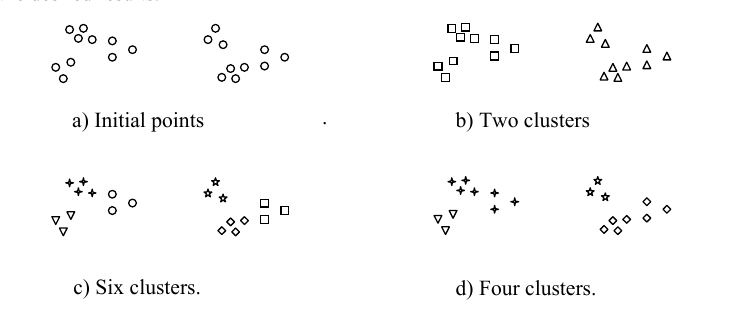
\includegraphics[width=0.8\textwidth]{img/howToCluster.png}
   \caption{}
   \label{res:img-howToCluster}
\end{figure}

En este trabajo para el agrupamiento se definió que cada grupo contenga la máxima cantidad de ítems sin exceder el presupuesto. La agrupación se realiza por la similitud de los objetos, que se obtiene a través de la \textbf{función de similitud}, para que los ítems dentro del grupo sean lo más parecidos posible y así obtener paquetes cohesivos.

En la literatura se pueden encontrar diferentes tipos de algoritmos de agrupamiento, la mayoría puede ser categorizado en particionales o jerárquicos \cite{opac-b1087461}. 

En los métodos de agrupamiento particional cada objeto es asignado a uno de los grupos posibles. La cantidad de grupos es establecida antes del inicio del proceso de agrupamiento. 

A diferencia de los métodos particionales, los jerárquicos construyen grupos mediante la partición recursiva de los grupos de objetos y no requieren predefinir una cantidad de grupos a generar. A su vez estas técnicas se suelen subdividir en dos estrategias: aglomerativas y divisivas, las cuales serán detalladas más adelante.

Se plantearán dos mejoras para el algoritmo jerárquico \textit{Constrained hierarchical agglomerative clustering} presentado en el artículo \cite{journals/tkde/Amer-YahiaBCFMZ14}: 
\begin{enumerate}
	\item La elección en cada iteración de la estrategia para combinar \textit{clusters}.
	\item La complejidad algorítmica.
\end{enumerate}

En las próximas secciones se describen detalladamente las mejoras propuestas.

El algoritmo \textit{BOBO}, descripto en \autoref{chap:trabajos-previos}, se mantuvo sin cambios en pos de realizar comparaciones entre los resultados obtenidos a través de las mejoras propuestas y las obtenidas mediante la implementación original.

\subsubsection{Bundles One-By-One}
El método \texttt{BOBO-k}, inspirado en \textit{k-means}, consiste en generar $k$ paquetes del conjunto de $n$ ítems. El algoritmo comienza con todos los ítems del conjunto $I$ como posibles pivotes $P$. Se selecciona un pivote de $P$ y con los elementos de $I$ se genera un paquete válido ``alrededor'' de éste; en caso que el paquete generado sea suficientemente bueno se agrega al conjunto de candidatos, en tanto los ítems del paquete se eliminan de $I$. La generación de paquetes continúa hasta que se cumpla el criterio de parada, que es generar $k$ paquetes válidos.

\begin{center}
	\begin{algorithm}[H]
	\DontPrintSemicolon
	\SetAlgoLined
		\KwData{$I,\alpha,f,\beta,\mu,\text{ cantidad de paquetes }c$}
		\KwResult{Conjunto válido de paquetes}
		$pivots \leftarrow I$\;
		$cand \leftarrow \emptyset$\;
		\While{$ \left|C\right| < c\ and\ pivots \neq \emptyset$}{
			$pivot \leftarrow SelectPivot(pivots)$\;
			$bundle \leftarrow BuildBundle(pivot,I,\alpha,f,\beta)$\;
			\eIf{$Score(bundle) \geq \mu$}{
				$cand \leftarrow cand \cup \left\{bundle\right\}$\;
				$I \leftarrow I \setminus \left\{bundle\right\}$\;
				$pivots \leftarrow pivots \setminus \left\{pivot\right\}$\;
			}
			{
				$pivots \leftarrow pivots \setminus \left\{pivot\right\}$\;
			}
		}
		\Return $cand$\;
	\caption{BOBO-k}\label{alg:bobo}
	\end{algorithm}
\end{center}

La función \texttt{selectPivote} selecciona un pivote perteneciente al conjunto de pivotes. En este trabajo se siguió con la recomendación citada en \cite{Zhang:2002:ESI:638644.638646}, la cuál dice que la selección sea aleatoria. La función \texttt{BuildBundle} genera un paquete a partir del pivote. Se trata de una función que implementa un algoritmo goloso, dado que en cada iteración se agrega al paquete que se genera el ítem del conjunto $I$ que maximiza la función intra y que cumple con las restricciones de complementariedad y presupuesto. La función \texttt{Score} calcula el valor intra del paquete. Se dice que un paquete es suficientemente bueno si el valor intra supera el umbral establecido por $\mu$.

\subsubsection{Constrained hierarchical agglomerative clustering}
Anteriormente se indicó que el agrupamiento jerárquico suele clasificarse en algoritmos \textit{aglomerativo} y \textit{divisivo}. 

El aglomerativo comienza con cada objeto perteneciente a un grupo unitario y en cada iteración se unen dos grupos generando un grupo nuevo. Este algoritmo es conocido como \textit{hierarchical agglomerative clustering} (HAC) \cite{journals/tkde/Amer-YahiaBCFMZ14}. 

La estrategia divisiva, en cambio, comienza con todos los objetos en un mismo grupo y en cada paso se realiza la división de uno de los grupos.

Comúnmente a los algoritmos algomerativos (HAC desde ahora en adelante) se los puede visualizar como un dendrograma, como se ve en la~\autoref{nuevaspropuestas:dendograma1}: en el eje X se encuentran los objetos que van a ser agrupados y en el eje Y se halla la distancia en la que los elementos se unirán. Las uniones de los objetos se representan mediante una línea vertical que comienza a la altura de la distancia en la que los grupos han sido unidos. Por ejemplo, en la figura mencionada, el grupo \textit{4} se une al \textit{5} en la distancia 2 formando el \textit{cluster B}. En un paso posterior éste último se unirá al grupo \textit{3} en una distancia cercana a 3 obteniendo el nuevo \textit{cluster C}. En cada paso se generará una nueva unión hasta que solo quede un único grupo.

\begin{figure}[H]
  \centering
    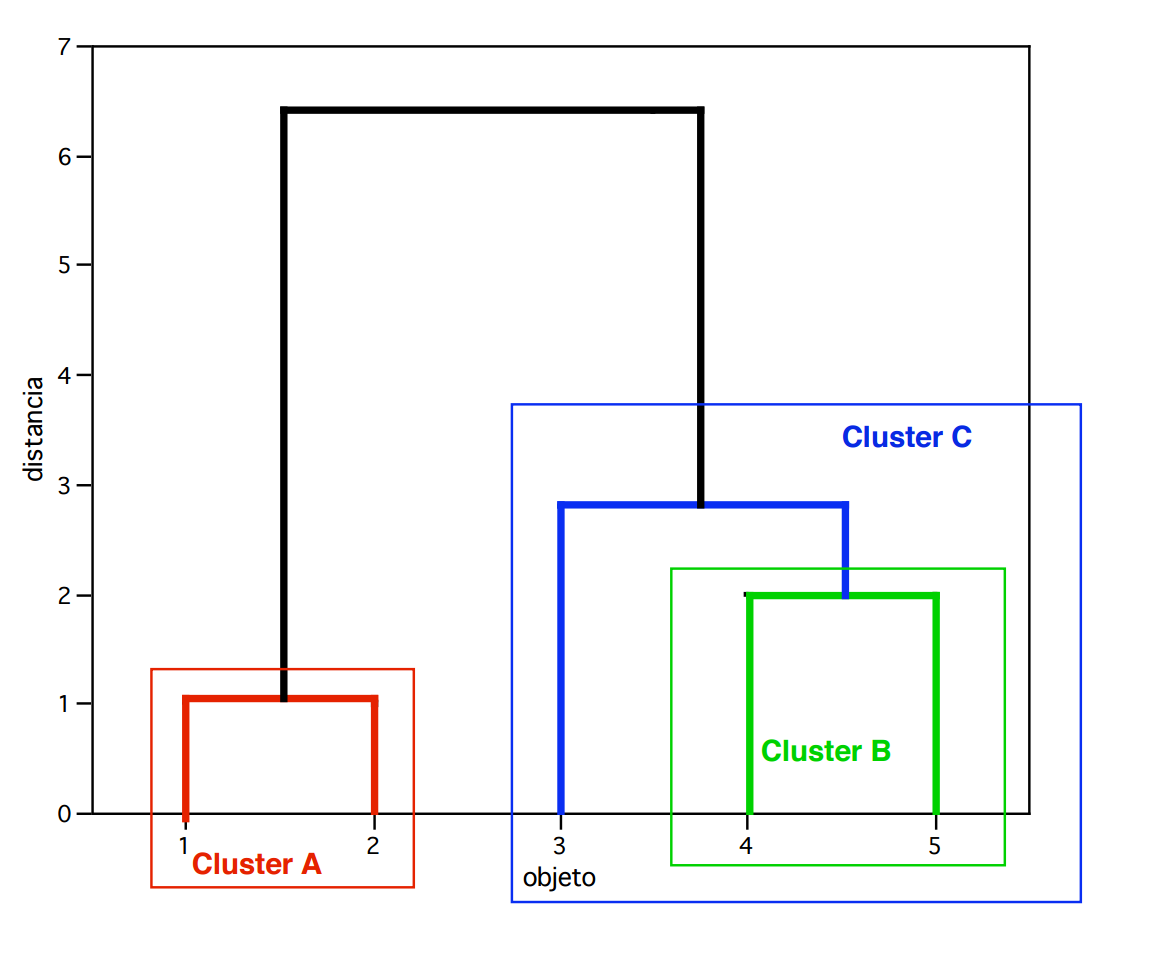
\includegraphics[width=0.5\textwidth]{img/dendograma01.png}
  \caption{Dendrograma}
  \label{nuevaspropuestas:dendograma1}
\end{figure}

Cortando el dendrograma mediante líneas horizontales se puede determinar el número de paquetes o \emph{clusters} en el que se dividirá el conjunto de objetos inicial. En la~\autoref{nuevaspropuestas:dendograma2} parte a) se puede ver que aplicando un corte en la distancia 5 se obtienen 2 paquetes, en cambio si se aplicara a una distancia mayor a 2 se obtendrían 3 paquetes, como puede observarse en la parte b) de la misma figura.

\begin{figure}[H]
  \centering
    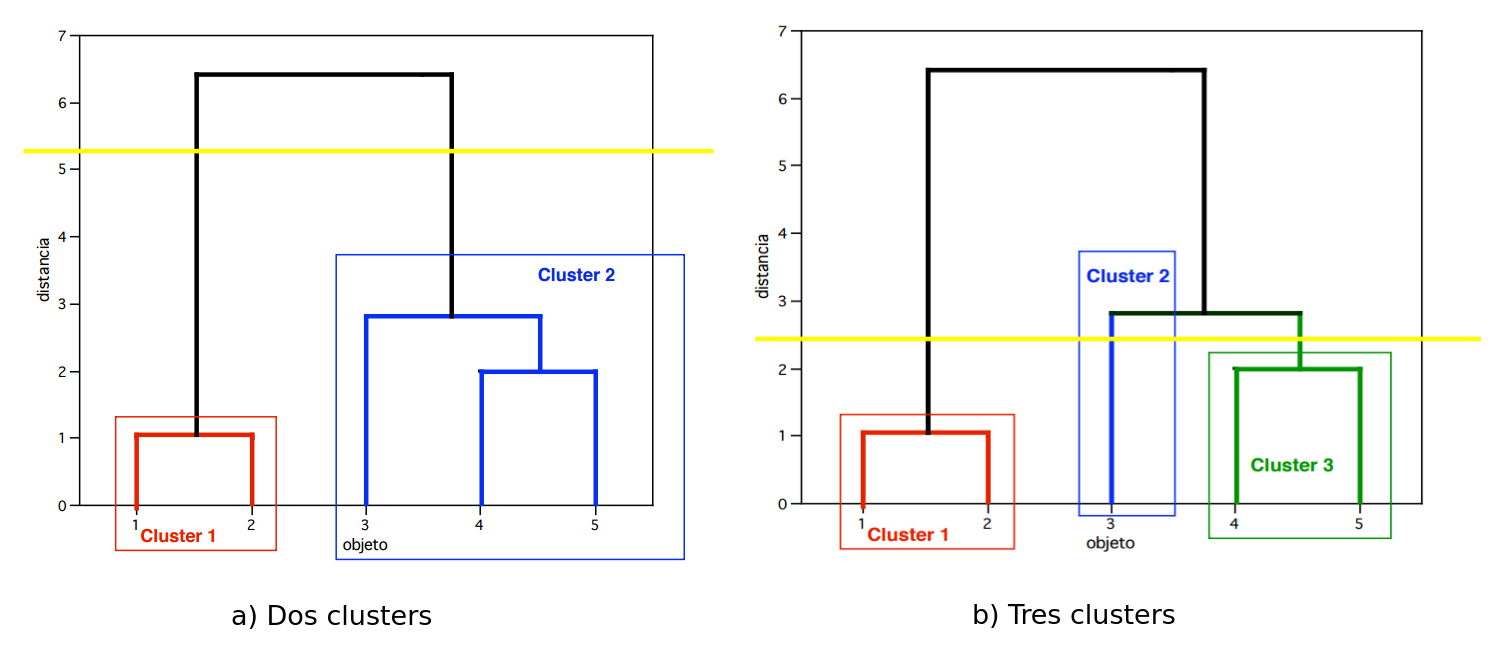
\includegraphics[width=1\textwidth]{img/dendograma02.png}
  \caption{Cortes en el dendrograma}
  \label{nuevaspropuestas:dendograma2}
\end{figure}

El algoritmo \textit{Constrained hierarchical agglomerative clustering} (C-HAC) presentado en \cite{journals/tkde/Amer-YahiaBCFMZ14}, se basa en el algoritmo HAC y tiene la particularidad que cada nuevo grupo que se genera en cada iteración (a partir de la unión de dos grupos) cumple con las restricciones de complementariedad y presupuesto. Por ejemplo, el algoritmo evalúa la unión de los grupos $S_1$ y $S_2$. Si el grupo resultante $S_1 \cup S_2$ es inválido, o sea, no cumple con las reglas recientemente mencionadas, entonces el algoritmo no aplicará dicho agrupamiento.

\begin{center}
	\begin{algorithm}[H]
	\DontPrintSemicolon
	\SetAlgoLined
		\KwData{$I,\alpha,f,\beta,\gamma,\text{ cantidad de paquetes }c$}
		\KwResult{Conjunto válido de paquetes}
		$cand \leftarrow \left\{\left\{i\right\}: i \in I\right\}$\; \label{alg:C-HAC:init}
		\While{$ \left|cand\right| > c$}{ \label{alg:C-HAC:cycleOutter}
			$bestScore \leftarrow -\infty$\;
			$bestCandidate \leftarrow \emptyset$\;
			\ForEach{$S_i\in cand$}{ \label{alg:C-HAC:cycleInner}
				\ForEach{$S_j\in cand; S_i \neq S_j$}{ \label{alg:C-HAC:cycleInnerInner}
					\If{$ValidMerge(S_i,S_j,\alpha,f,\beta)$}{ \label{alg:C-HAC:validMerge}
						\If{$Score(S_i \cup S_j) \geq bestcore$}{ \label{alg:C-HAC:score}
							$bestScore \leftarrow Score(S_i \cup  S_j)$\;
							$bestCandidate \leftarrow \left\{S_i,S_j\right\}$\;
						}
					}
				}
			}
			\If{$bestCandidate = \emptyset$}{
				$break$\;
			}
			$cand \leftarrow cand \setminus \left\{S\right\}$ $(\forall S \in bestCandidate)$\;
			$cand \leftarrow cand \cup bestCandidate$\;
		}
		\Return $cand$\;
	\caption{C-HAC}\label{alg:C-HAC}
	\end{algorithm}
\end{center}

Analizando la complejidad del\textbf{~\autoref{alg:C-HAC}} el principal ciclo se ejecuta $N - c$ veces, donde $N$ es la cantidad de ítems. En cada paso de la iteración principal se unirán los dos conjuntos con mayor similitud y que el conjunto resultante de esa unión sea válido. 

Cada uno de los ciclos interiores (\textit{~\autoref{alg:C-HAC:cycleInner} y~\autoref{alg:C-HAC:cycleInnerInner}}) itera sobre los elementos contenidos en el conjunto de grupos candidatos a unir, realizando comparaciones entre todos los grupos existentes hasta el momento. 

La función \textit{Score} que se utiliza para decidir qué {\em clusters} unir, sólo toma en cuenta el valor \texttt{intra}, por lo que dicha operación puede ser tratada como constante, ya que se trata de un número fijo de comparaciones. Lo mismo pasa con la función que valida la unión de los conjuntos \texttt{ValidMerge}.

Tomando como peor caso que cada iteración tenga $N$ pasos, el orden de complejidad de \texttt{C-HAC} es $\mathcal{O}(N^{3})$. 

Para que la dispersión de los paquetes que se generan en la fase de producción coincida con la esperada por el usuario se decidió en esta tesis, modificar el algoritmo \texttt{C-HAC} para incluir el valor \texttt{inter} en el cálculo de la selección del par de grupos que se une. De esta manera, al evaluar la unión entre dos grupos se considera tanto el valor \texttt{intra} como también así la distancia con el resto de los paquetes del posible nuevo paquete. A diferencia de la función \textit{Score} vista previamente, en la que solo tenía en cuenta el valor \texttt{intra}, se definió la función \textit{Intra-Inter} en la que ambas partes de la función objetivo son tenidas en consideración. 

Entonces, para \textit{Intra-Inter} dados dos {\em clusters} $C_i$ y $C_j$ sean

$$A(C_i,C_j) = \sum_{u \in C_i, v \in C_j}{s(u,v)},$$

$$E(C_i,C_j)=\max_{u \in C_i, v \in C_j}{s(u,v)} \qquad \mbox{ y}$$

$$\mbox{Intra-Inter}(C_i,C_j) = \gamma A(C_i,C_j) + t (1-\gamma) E(C_i,C_j)$$

De esta manera el {\em cluster} resultante incrementará el valor \texttt{inter} y se habrán unido dos {\em clusters} con alta similitud, favoreciendo la dispersión en el {\em clustering} final. El factor $t$ intenta equilibrar los dos términos de la sumatoria, de lo contrario, el segundo resultará siempre despreciable con respecto al primero. Por lo tanto se decidió que el valor que se le asigna a $t$ corresponde a la cantidad de similitudes que se suman en A, o sea $\frac{(\#C_i + \#C_j) (\#C_i + \#C_j - 1)}{2}$  

Si bien el objetivo principal de la modificación propuesta es aumentar la calidad de las soluciones, también se tuvo en cuenta la complejidad temporal del algoritmo. De lo contrario, el uso de las mejoras no hubieran podido ser usadas en las pruebas, que se detallarán en los próximos capítulos, por tratarse de instancias con miles de objetos.

En \textbf{~\autoref{alg:Intra-Inter C-HAC}}, \texttt{Intra-Inter C-HAC}, se muestra el procedimiento propuesto en esta tesis para producir paquetes. Este algoritmo mejora la calidad, el cual mejora la complejidad de  \texttt{C-HAC} e incluye la información inter-paquete. La complejidad de este nuevo algoritmo es $\mathcal{O}(n^{2}\log n)$. 

\texttt{Intra-Inter C-HAC} cuenta principalmente con dos estructuras. La matriz $C$, que en la posición $i,j$ almacena la similitud de los grupos $i$ y $j$, y un arreglo de colas de prioridad, donde la cola $P_i$ contiene (en orden decreciente) la relación de similitud del grupo $i$ con el resto de los grupos.

El algoritmo comienza con la inicialización de la matriz $C$ de tamaño $n$ $x$ $n$ y con el arreglo de colas de prioridad $P\left[n\right]$, donde $n$ es la cantidad de elementos. Como ya se había anticipado \texttt{Intra-Inter C-HAC} es un algoritmo jerárquico divisivo, por lo que en la inicialización de $C$ en la posición $i,j$ se almacena el valor de la similitud del grupo unitario $i$ $j$.

Luego de la inicialización de las estructuras, \texttt{Intra-Inter C-HAC} continúa con un ciclo en el que en cada iteración se obtiene entre todas las colas con $P\left[k\right].max()$ el grupo con mayor grado de similitud. Siendo $\omega_{k_{1}}$ y $\omega_{k_{2}}$ los grupos con mayor similitud, se realiza la unión entre estos y se utiliza $\omega_{k_{1}}$  como la representación de la unión. Para el nuevo  $\omega_{k_{1}}$ se calcula la similitud con el resto de los grupos y se actualiza en las colas de similitud.

\begin{center}
	\begin{algorithm}[H]
	\DontPrintSemicolon
	\SetAlgoLined
		\KwData{$I,\alpha,f,\beta,\gamma$}
		\KwResult{Conjunto válido de paquetes}
		\ForEach{$S_i\in I$}{
			\ForEach{$S_j\in I$}{
				\eIf{$validMerge(S_i,S_j,\alpha,f,\beta)$}{
					$C[i][j].sim \leftarrow Score(S_i \cup S_j)$\;
				}
				{
					$C[i][j].sim \leftarrow -1$\;
				}
				$C[i][j].index \leftarrow j$\;
			}
			$I[i] \leftarrow 1$\;
			$P[i] \leftarrow $ priority queue for $C[i]$ sorted on sim\;
			$P[i].Delete(C[i][i])$ \tcc*[f]{se elimina así mismo de la pila}\;
		}
		$A \leftarrow []$\;
		\For{$n \leftarrow 1$ to $I.length$}{
			$k_1 \leftarrow \max_{k:I[k]=1}{P[k].max().sim}$\;
			\If{$validMerge(S_i,S_j,\alpha,f,\beta)$}{
				$break$\;
			}
			$k_2 \leftarrow P[k_1].max().index$\;
			$A.Append(\left\langle k_1,k_2 \right\rangle)$\;
			$I[k_2] \leftarrow 0$\;
			$P[k_1] \leftarrow []$\;
			\For{$i$ with $I[i]-1 \vee i \neq k_1$}{
				$P[i].Delete(C[i][K_1])$\;
				$P[i].Delete(C[i][k_2])$\;
				\eIf{$validMerge(S_i,S_j,\alpha,f,\beta)$}{
					$C[i][k_1].sim \leftarrow Inter-Intra(i,k_1 \cup k_2,\gamma)$\;
					$C[k_1][i].sim \leftarrow Inter-Intra(i,k_1 \cup k_2,\gamma)$\;
				}
				{
					$C[i][k_1].sim \leftarrow -1$\;
					$C[k_1][i].sim \leftarrow -1$\;
				}
				$C[i][k_1].index \leftarrow i$\;
				$C[k_1][i].index \leftarrow i$\;
				$P[i].Insert(C[i][k_1])$\;
				$P[K_1].Insert(C[k_1][i])$\;
			}
		}
		\Return $A$\;
	\caption{Intra-Inter C-HAC}\label{alg:Intra-Inter C-HAC}
	\end{algorithm}
\end{center}

Retomando las fórmulas presentadas anteriormente, para evitar recalcular en cada iteración los valores ya calculados, se redefinen las fórmulas $A$ y $E$ de forma recursiva. De esta manera para la implementación se mantienen estructuras con esos valores, por lo que la complejidad de la función \textit{Intra-Inter} es constante. A partir de las relaciones entre la iteración $r$ y $r-1$ se tiene que:

$$A^r(C_i \cup C_j, C_s) = A^{r-1}(C_i,C_s) + A^{r-1}(C_j,C_s) \quad \mbox{ y}$$

$$E^r(C_i \cup C_j,C_s) = \max (E^{r-1}(C_i,C_s),E^{r-1}(C_j,C_s))$$

El ciclo de la inicialización de las estructuras es $\mathcal{O}(n^{2})$. Mientras que el ciclo de unión de conjuntos es $\mathcal{O}(n^{2}\log n)$ para una implementación de las colas de prioridad en que la inserción y borrado es $\mathcal{O}(\log n)$. La complejidad final del algoritmo es $\mathcal{O}(n^{2}\log n)$.

\subsection{Mejoras en la selección de paquetes}
En \emph{Produce and Choose} luego de la producción de paquetes se realiza la selección del subconjunto de paquetes que será la solución. A continuación se detallará el comportamiento de la implementación original de \cite{journals/tkde/Amer-YahiaBCFMZ14} y los cambios propuestos.

El problema puede representarse como un grafo completo con pesos en las aristas y vértices. 

Los nodos corresponden a los paquetes generados en la primera parte del algoritmo y su peso equivale a su calidad o valor \texttt{intra}. Las aristas representan la distancia existente entre los nodos y su peso está definido en el valor \texttt{inter} de los paquetes involucrados. Teniendo en cuenta la transformación mencionada se puede interpretar que la solución de encontrar aquellos paquetes que maximicen la función objetivo es equivalente a encontrar un k-subgrafo completo de mayor peso.

La definición formal de encontrar el subgrafo completo de tamaño k de peso máximo entre nodos y vértices es la siguiente: dado el grafo $ G = (V,E) $, las funciones de peso $\psi : E \rightarrow \Re$ y $\omega : V \rightarrow \Re$, el entero $ k \leq |V| $ y el real $\gamma \in [0,1]$. 

El resultado es el conjunto $V' \subseteq V$ tal que $|V'| = k$ y que maximiza el peso de los nodos y vértices del subgrafo $G' = (V', E')$ ponderado por el parámetro $\gamma$.

\begin{equation}
\gamma \sum_{v \in V'}{\omega(v)} + (1 - \gamma) \sum_{(u,v) \in E'}{\psi(u,v)}
\end{equation}

El problema previamente mencionado puede reducirse a la conocida situación de hallar el k-subgrafo más denso \cite{DBLP:journals/algorithmica/FeigePK01} transformando el grafo del problema original a un grafo ponderado, en el que el peso de los vértices está dado por la siguiente función:
 
\begin{equation}
\omega(u,v) = \dfrac{\gamma}{2( k - 1)} (\omega(u) + \omega(v)) + (1 - \gamma)\psi(u,v) 
\end{equation}

En \cite{journals/tkde/Amer-YahiaBCFMZ14} proponen utilizar como heurística el algoritmo \ref{alg:chooseBundles} para hallar el k-subgrafo de mayor peso de un grafo ponderado. El algoritmo en cada iteración, elimina un vértice al par de nodos con menor peso del grafo, hasta que quedarse con un grafo de $k$ nodos.

\begin{center}
	\begin{algorithm}[H]
	\DontPrintSemicolon
	\SetAlgoLined
		\KwData{$k,\gamma,\text{ el grafo con peso en los vértices y aristas }G=(V,E) \text{ donde }\forall S \in V / \omega(S) = \sum_{u,v \in S}{s(u,v)}$ y $\forall (S_i,S_j) \in E / \psi(S_i,S_j) = 1 - \max_{u \in S_i, v \in s_j}{s(u,v)}$}
		\KwResult{Conjunto de k bundles}
		$\omega(u,v) = \dfrac{\gamma}{2( k - 1)} (\omega(u) + \omega(v)) + (1 - \gamma)\psi(u,v)$\;
		$S \leftarrow V$\;
		\While{$ \left|S\right| > k$}{
			$u \leftarrow \min_{u \in S}{\sum_{v \in S}{\omega(u,v)}}$\;
			$S \leftarrow S \setminus  \left\{u\right\} $\;
		}
		\Return $C$\;
	\caption{Selección de paquetes}\label{alg:chooseBundles}
	\end{algorithm}
\end{center}


 

La debilidad de este algoritmo reside en que para seleccionar el próximo nodo a remover (paquete) no se considera el \textit{valor} del nodo (valor intra). Entonces se puede dar el caso de que el nodo que se remueve pertenezca una solución de mejor calidad.

Por ejemplo si se considera que en la etapa de producción se generan los tres paquetes $A$, $B$ y $C$, en el cual el valor \texttt{Intra} para cada uno de los paquetes es: $\omega(A) = 5$, $\omega(B) = 5$ y $\omega(C) = 5$ y el valor \texttt{Inter} entre los paquetes: $\psi(A,B) = 0$, $\psi(A,C) = 1$ y $\psi(B,C) = 0$. En este escenario para la solución que contenga dos paquetes y con $\gamma=0,1$ se tiene los siguientes valores para cada par de paquetes:
\begin{itemize}
	\item $\omega(A,B) = 0,45$
	\item $\omega(A,C) = 1,15$
	\item $\omega(B,C) = 0,2$
\end{itemize}
 
El par de paquetes $B, C$ es el que tiene el menor valor en la función $\omega$, por lo tanto, si el paquete elegido para ser eliminado es $C$ y la solución resultante contendrá a los paquetes $A$ y $B$. 

El valor de la función objetivo de esta solución generada es $0,9$, mientras que el valor de la función objetivo de la solución que contiene a los paquetes $A$ y $C$ es $1,4$.

Tomando esto como base, se propone un nuevo enfoque para seleccionar los paquetes de la solución. A diferencia del algoritmo anterior, la solución se genera iterativamente agregando en cada paso el paquete que maximiza la función objetivo hasta alcanzar la cantidad de paquetes requeridos en la solución.

Para los paquetes generados en el ejemplo anterior, las soluciones posibles en la primera iteración son $S^{1}_{1}=\{A\}$, $S^{1}_{2}=\{B\}$ y $S^{1}_{3}=\{B\}$. Dado que $S^{1}_{1}$ es el candidato con mayor valor de función objetivo, se selecciona este y para la segunda iteración las posibles elecciones son:  $S^{2}_{1}=\{A,B\}$, $S^{2}_{2}=\{A,C\}$. Quedándose finalmente con la solución $S^{2}_{2}$ que, como se vio anteriormente, es la de mayor función objetivo.

En los casos estudiados, la relación entre la parte \texttt{intra} y la \texttt{inter} de la función objetivo es que el valor de la parte \texttt{intra} es considerablemente mayor que el \texttt{inter}. Esto se debe a que en un paquete el valor \texttt{intra} está dado por la suma de todas las similitudes entre los elementos del paquete, mientras que el valor de la parte \texttt{inter} es de solo una de las relaciones. Además, entre una solución $S'$ que contiene $n$ paquetes y la solución $S''$ que contiene $n+1$ paquetes, $S''$ tiene $n$ relaciones inter-paquete más que $S'$. 

A continuación se propone una función para este nuevo algoritmo en el que se compensan estas diferencias.

El algoritmo \ref{alg:algSelProp} en la etapa de selección utiliza una función, que es una variante de la función objetivo, para seleccionar en cada iteración el paquete que formará parte de la solución. En la variante cada parte de la función objetivo es multiplicada por un coeficiente \textbf{coef}. Con este coeficiente se equilibra la parte \texttt{intra} y la \texttt{inter} durante todo la generación de la solución.   

Formalmente esta función se define de la siguiente manera. Sea $R$ el conjunto de paquetes producidos y $S \subseteq R$ el conjunto de paquetes seleccionados en la iteración $i$, se agrega a la solución el paquete que cumple con:

\begin{equation}
\max_{b \in (R/S)}{\dfrac{k}{|S|}} \gamma \sum_{v \in \left\{b\right\} \cup S}{\omega(v)} + \dfrac{k * (k-1)}{|S| * (|S|-1)} (1-\gamma) \sum_{v,w \in \left\{b\right\} \cup S}{\psi(v,w)}
\end{equation}

\begin{center}
	\begin{algorithm}[H]
	\DontPrintSemicolon
	\SetAlgoLined
		\KwData{$k,\gamma, \text{el grafo con peso en los vértices y aristas } G=(V,E) \text{ donde } \forall S \in V / \omega(S) = \sum_{u,v \in S}{s(u,v)} y \forall (S_i,S_j) \in E / \psi(S_i,S_j) = 1 - \max_{u \in S_i, v \in s_j}{s(u,v)}$}
		\KwResult{Conjunto de k bundles}
		$\omega(u,v) = \dfrac{\gamma}{2( k - 1)} (\omega(u) + \omega(v)) + (1 - \gamma)\psi(u,v)$\;
		$S \leftarrow \emptyset$\;
		$R \leftarrow V$\;
		\While{$ \left|S\right| < k$}{
			$c \leftarrow \max_{b \in (R/S)}{\dfrac{k}{|S|}} \gamma \sum_{v \in \left\{b\right\} \cup S}{\omega(v)} + \dfrac{k * (k-1)}{|S| * (|S|-1)} (1-\gamma) \sum_{v,w \in \left\{b\right\} \cup S}{\psi(v,w)}$\;
			$S \leftarrow S \cup \left\{c\right\}$\;
			$R \leftarrow R \setminus \left\{c\right\}$\;
		}
		\Return $S$\;
	\caption{Selección de paquetes proporcional}\label{alg:algSelProp}
	\end{algorithm}
\end{center}

\section{Resolución con algoritmo goloso}

Para el problema de \texttt{Recuperación de Ítems Empaquetados} se propone una solución basada en heurísticas golosas, la cual abordará dos temas puntuales:
\begin{itemize}
	\item Que la solución se construya teniendo la misma consideración sobre las dos partes de la función objetivo -la parte \texttt{inter} y la \texttt{intra}- durante todo el proceso.
	\item Que sea aceptable el tiempo de ejecución para grandes cantidades de ítems.
\end{itemize}

El objetivo del primer punto es proponer una variante a \texttt{Produce-and-choose}. Las soluciones que se generan con \texttt{Produce-and-choose} están más enfocadas en la parte \texttt{intra}, porque primero produce paquetes sin considerar la parte \texttt{inter} de la función objetivo.

Un algoritmo goloso es un tipo de heurística que construye la solución iterativamente seleccionando en cada paso la mejor opción local, esperando así lograr una solución óptima. En la mayoría de los problemas el algoritmo goloso no encuentra la solución de buena calidad, pero son muy usados por su sencillez y velocidad de ejecución.

Por los motivos mencionados y por las características del algoritmo goloso, se decidió implementar esta heurística para encontrar una solución. 

El algoritmo goloso que se propone, comienza con los $k$ paquetes de la solución vacíos, y en cada iteración se agrega un ítem que no pertenece a la solución, ubicándolo en el paquete que maximiza la función objetivo, sin violar las restricciones del problema. El algoritmo finaliza cuando por alguna restricción no es posible agregar más objetos a la solución. Sea $I$ el conjunto de ítems del problema, $\omega$ la función objetivo y en el inicio la solución $S_0 = \emptyset$ y $t=1$ entonces se define $S_t = S_{t-1} \cup \{i\}$ dónde $i \in I$, $i \notin S_{t-1}$ y $S_t$ es una solución válida. 

Como se puede ver, esta implementación prioriza la cantidad de elementos de la solución, ante el valor objetivo de la misma. Con esto se quiere decir que en cada paso, si es posible, se agrega un ítem a la solución, pese a que disminuya el valor de la función objetivo. Por lo que un escenario posible es que $\omega(S_{t-1}) > \omega(S_t)$.

\begin{center}
	\begin{algorithm}[H]
	\DontPrintSemicolon
	\SetAlgoLined
		\KwData{$I,\alpha,f,\beta,k,\gamma$}
		\KwResult{Conjunto válido de paquetes}
		$\omega(S) = \sum_{b \in S}{\sum_{u,v \in b}{\gamma s(u,v)}} + \sum_{b_1,b_2 \in S}{(1-\gamma) (1-\max_{u \in b_1, v \in b_2}{s(u,v)})}$\;
		$cand \leftarrow \bigcup_{1 \ldots k}\emptyset$\;
		$isComplete \leftarrow False$\;
		\While{$isComplete = False$}{
			$bestScore \leftarrow -\infty$\;
			$bestCandidate \leftarrow \varnothing$\;
			$bestBundle \leftarrow \varnothing$\;
			\ForEach{$elem \in I$}{
				\ForEach{$bundle \in cand$}{
					\If{$validMerge(bundle,\{elem\},\alpha,f,\beta)$}{
						$score \leftarrow \omega((Cand \setminus \left\{bundle\right\}) \cup \left\{bundle \cup \left\{elem\right\}\right\})$\;
						\If{$score > bestScore$}{
							$bestScore \leftarrow score$\;
							$bestBundle \leftarrow bundle$\;
							$bestCandidate \leftarrow elem$\;
						}
					}
				}
			}
			\eIf{$bestCandidate \neq \varnothing$}{
				$cand \leftarrow (cand \setminus \left\{bestBundle\right\}) \cup \left\{bundle \cup \left\{bestCandidate\right\}\right\}$\;
				$I \leftarrow I \setminus \left\{bestCandidate\right\}$\;
			}{
				$isComplete \leftarrow True$\;
			}
		}
		\Return $cand$\;
	\caption{Algoritmo heurística golosa}\label{alg:algHeuGol}
	\end{algorithm}
\end{center}

\section{Resolución con Búsqueda Tabú}
Pretendiendo mejorar las soluciones que se obtuvieron hasta el momento, conservando las premisas del tamaño del conjunto de ítems y el tiempo de ejecución acorde con el resto de los algoritmos, se implementaron distintas variantes de la metaheurística \textbf{Tabú search}. 

\textbf{Tabú search} \cite{TS-1,TS-2} es una metaheurística para resolver problemas de optimización, de la familia de las búsquedas locales, diseñada para escapar de óptimos locales. Se basa en buscar una mejor solución a partir de una anterior existente, lo que permite ser combinada junto con las heurísticas estudiadas anteriormente. 

Las búsquedas locales consisten en moverse de una solución a otra, aplicando cambios a la solución candidata hasta encontrar una mejor o satisfacer un criterio de parada. 

Los algoritmos comienzan a partir de una instancia válida, que puede haber sido obtenida mediante algún otro método, y en cada iteración se mueve a una solución vecina, esto es posible sólo si se puede definir una relación de vecindad entre las instancias del problema. Como una solución puede tener muchas instancias vecinas, se elige siempre aquella que maximice (o minimice, según el problema elegido) el criterio seleccionado, produciendo que el algoritmo pueda estancarse en un máximo (ó mínimo) local y nunca pueda salir de él.

Para explorar regiones del espacio de búsqueda, que serían dejadas de lado por el procedimiento de búsqueda local, la búsqueda tabú permite moverse a una solución vecina de menor calidad modificando la estructura de vecinos en cada una de las soluciones. De esta manera, se permite al algoritmo escapar de máximos (o mínimos) locales.

Las implementaciones de búsqueda tabú utilizan estructuras de memoria, conocidas como \textbf{listas tabú}, que determinan cuáles son las soluciones vecinas permitidas de una instancia. Para evitar que soluciones de buena calidad no sean visitadas porque la lista tabú lo prohíbe, se introduce el concepto de criterios de aspiración, que permite bajo ciertas circunstancias, eludir las restricciones tabú y así poder visitar soluciones.

Se implementaron las búsquedas tabú Inter-Paquete e Intra-Paquete. Una busca encontrar una mejor solución entre la actual y los paquetes ya generados. La otra consiste en mejorar los paquetes con los ítems que quedaron fuera de la solución.

\subsection{Inter-Paquete}
La búsqueda \texttt{Inter-Paquete} se diseñó especialmente para el algoritmo \texttt{Produce and Choose}. La idea surge de aprovechar los paquetes generados que no forman parte de la solución. Es por eso que se plantea un búsqueda tabú que comienza con una solución inicial obtenida a través de \texttt{Produce and Choose} y luego se intenta buscar una mejor con los paquetes que no pertenecen a la instancia inicial. 

Para esta implementación se define que las instancias vecinas de la solución $S$, son aquellas que no contienen al paquete con menor valor Inter de $S$ e incluye a un paquete que no pertenece a $S$. El paquete que se saca de $S$ se agrega a la lista tabú durante una cantidad establecida de iteraciones. Esta lista contiene los paquetes que no pueden ser parte de la próxima solución a visitar. Se elige entonces como criterio de aspiración, la admisión de una solución vecina que contiene un paquete que está en la lista tabú, si mejora la función objetivo con respecto a la mejor solución encontrada hasta el momento. 

El esquema del proceso para construir una nueva solución es el siguiente:

\begin{enumerate}
\item $S^* = S$, $ \bar{S}= S$, $LT = \emptyset$

\item Mientras no se cumpla criterio de parada hacer:

\begin{enumerate}
      	
\item Identificar el paquete $b_r$ en $\bar{S}$ con menor inter:

$$b_r = \argmin_{\scriptscriptstyle b_i \in \bar{S}} \sum_{\substack{\scriptscriptstyle  b_j \in \bar{S} \\ \scriptscriptstyle  b_j \ne b_i}} (1-\max_{\substack{\scriptscriptstyle  u\in b_i \\ \scriptscriptstyle v \in b_j}} s(u,v))$$

\item Determinar el paquete, $b_c$, con menor inter en $\bar{S} \setminus \{b_r\}$
	
\item Determinar el conjunto de paquetes candidatos $C$ como los paquetes de $B\setminus \bar{S}$ que maximizan su inter respecto a $b_c$:

$$C = \argmax_{\scriptscriptstyle b_i \in B \setminus \bar{S}} (1-\max_{\substack{\scriptscriptstyle u\in b_i \\ \scriptscriptstyle v \in b_c}} s(u,v))$$

\item Determinar el mejor paquete de $C$ no prohibido en la lista tabú $LT$ según el criterio:

$$b = \argmax_{\scriptscriptstyle b_s \in C \setminus LT} \sum_{\scriptscriptstyle b_i, b_j \in \bar{S}\setminus \{b_r\} \cup \{b_s\}}(1-\max_{\substack{\scriptscriptstyle u\in b_i \\ \scriptscriptstyle v \in b_j}} s(u,v))$$

\item Evaluar el criterio de aspiración para los paquetes en $C \cap LT$

$$b_{tabu} = \argmax_{\scriptscriptstyle b_s \in C \cap LT} w(\bar{S} \setminus \{b_r\} \cup \{b_s\})$$

\item Si $\max(w(S^*),w(\bar{S} \setminus \{b_r\} \cup \{b\})) < \qquad \qquad$ $\qquad \qquad w(\bar{S} \setminus \{b_r\} \cup \{b_{tabu}\})$ entonces

$$\bar{S} = \bar{S} \setminus \{b_r\} \cup \{b_{tabu}\}$$ 

Si no $$\bar{S} = \bar{S} \setminus \{b_r\} \cup \{b\}$$

\item Actualizar $LT$

\item Si $w(\bar{S})>w(S^*)$ entonces $S^*=\bar{S}$

\end{enumerate}

\item Retornar $S^*$

\end{enumerate}

\begin{center}
	\begin{algorithm}[H]
	\DontPrintSemicolon
	\SetAlgoLined
		\KwData{$S, cand, \gamma, MAX\_ITER, ITER\_TABU$}
		\KwResult{Conjunto válido de paquetes}
		$\omega(S) = \sum_{b \in S}{\sum_{u,v \in b}{\gamma s(u,v)}} + \sum_{b_1,b_2 \in S}{(1-\gamma) (1-\max_{u \in b_1, v \in b_2}{s(u,v)})}$\;
		$UpdateTabu(S) = \left\{ \left\langle b, n-1 \right\rangle  / \left\langle b, n \right\rangle \in S \wedge n-1 > 0 \right\}$\;
		$Inter(b_1, S) = \sum_{b_2 \in S, b_1\neq b_2}{(1-\max_{u \in b_1, v \in b_2}{s(u,v)})}$\;
		$Inter(S) = \sum_{b_1, b_2 \in S}{(1-\max_{u \in b_1, v \in b_2}{s(u,v)})}$\;
		$iteration \leftarrow 0$\;
		$tabuBundles \leftarrow \emptyset$\;
		$bestSolution \leftarrow S$\;
		$visitSolution \leftarrow S$\;
		\While{$iteration < MAX\_ITER$}{
			$worstBundle \leftarrow \min_{b \in visitSolution \setminus tabuBundles}{Inter(b, visitSolution)}$\;
			$centroidBundle \leftarrow getCentroid(visitSolution)$\;
			$visitSolution_a \leftarrow \max_{b \in cand}{(visitSolution \setminus \left\{worstBundle\right\}) \cup \left\{b\right\}}$\;
			$visitSolution \leftarrow \max_{b \in cand \setminus tabuBundles}{(visitSolution \setminus \left\{worstBundle\right\}) \cup \left\{b\right\}}$\;
			\If{$\omega(visitSolution) > \omega(bestSolution)$}{
				$bestSolution \leftarrow visitSolution$\;
			}
			\If{$\omega(visitSolution_a) > \omega(bestSolution)$}{
				$bestSolution \leftarrow visitSolution_a$\;
				$visitSolution \leftarrow visitSolution_a$\;
			}
			$tabuBundles \leftarrow tabuBundles \cup \left\{\left\langle worstBundle, ITER\_TABU \right\rangle\right\}$\;
			$tabuBundles \leftarrow UpdateTabu(tabuBundles)$\;
			$iteration \leftarrow iteration + 1$\;
		}
		\Return $bestSolution$\;
	\caption{Búsqueda tabú sobre paquetes}\label{alg:algBusTabuBundle}
	\end{algorithm}
\end{center}

\subsection{Intra-Paquete}
El objetivo de la búsqueda Intra-Paquete es buscar una mejor solución con paquetes más cohesivos. En esta búsqueda los vecinos de la solución $S$ son aquellos a los cuales se les modifica un paquete con alguna de las siguientes acciones: agregar un elemento, quitar un elemento o intercambiar un elemento del paquete con otro elemento que no pertenece a la solución. 

Para esta implementación existen tres listas tabú: 
\begin{enumerate}
	\item Una lista de elementos.
	\item Una de movimientos.
	\item Una de paquetes.
\end{enumerate}

Los elementos que se encuentran en la lista tabú, no pueden ser seleccionados para incluirse en una solución. Los paquetes de la lista son los que no pueden ser seleccionados para generar una nueva solución. La lista de movimientos contiene el par de elementos que se intercambiaron para ir de la solución $S$ a $S'$, a fin de que esos elementos no se vuelvan a intercambiar.

La lista de los movimientos se utiliza para evitar ciclar entre las soluciones. Por ejemplo si las soluciones visitadas son $S, S_1, \ldots, S_n, S$, la lista prohíbe que se vuelvan a intercambiar el mismo par de elementos y así asegura que la próxima no sea $S_1$.

El criterio de aspiración que se utiliza, es permitir elegir un elemento de la lista tabú para ser intercambiado por un elemento de la instancia actual, sólo si el valor de la función objetivo es mayor que el valor de la mejor solución encontrada hasta al momento.

Desde la solución actual se realiza el movimiento a una nueva solución con los siguientes pasos:

Sea $S$ el conjunto de paquete de la solución e $I$ el conjunto de ítems, el paquete de (1) es $b = \min_{b_1 \in S}{\sum_{v,w \in b_1}{s(v,w)}}$. De $b$ se define el centroide $c$ del paso (2) con $c = \max_{v \in b}{\sum_{w \in b}{s(v,w)}}$. El ítem de (3) se obtiene de $i = \min_{v \in b}{s(v,c)}$. El ítem para reemplazar a $i$ es $j = \max_{v \in I \setminus items(S)}{s(v,c)}$.

\begin{enumerate}
	\item Obtener el paquete, $p$, menos cohesivo de la solución $S$.
	\item Crear el paquete $p'$ válido agregando a $p$ un elemento que no pertenezca a la solución y no esté en la lista tabú.
	\item Crear el paquete $p''$ válido quitando de $p$ el elemento más alejado del centroide.
	\item Crear el paquete $p'''$ válido quitando de $p$ el elemento más alejado del centroide y agregando el elemento que no pertenece a la solución $S$ y no esté en la lista tabú.
	\item Crear el paquete $p''''$ válido quitando de $p$ el elemento más alejado del centroide y agregando el elemento que no pertenece a la solución $S$
	\item Sea $S_{i} = S\setminus \{p\}$, entonces la solución vecina que se visita es $S'$\\
	$S' = \argmax {FO(S_{i}\cup\{p'\}), FO(S_{i}\cup\{p''\}), FO(S_{i}\cup\{p'''\}), FO(S_{i}\cup\{p''''\})}$.
\end{enumerate}

\begin{center}
	\begin{algorithm}[H]
	\DontPrintSemicolon
	\SetAlgoLined
		\KwData{$S, cand, I, \alpha, f, \beta, k, \gamma, MAX\_ITER, ITER\_TABU$}
		\KwResult{Conjunto válido de paquetes}
		$\omega(S) = \sum_{b \in S}{\sum_{u,v \in b}{\gamma s(u,v)}} + \sum_{b_1,b_2 \in S}{(1-\gamma) (1-\max_{u \in b_1, v \in b_2}{s(u,v)})}$\;
		$Inter(b_1, S) = \sum_{b_2 \in S, b_1\neq b_2}{(1-\max_{u \in b_1, v \in b_2}{s(u,v)})}$\;
		$Intra(b) = \sum_{u,v \in b}{\gamma s(u,v)}$\;
		$UpdateTabu(S) = \left\{ \left\langle b, n-1 \right\rangle  / \left\langle b, n \right\rangle \in S \wedge n-1 > 0 \right\}$\;
		$iteration \leftarrow 0$\;
		$tabuBundles \leftarrow \emptyset$\;
		$tabuElements \leftarrow \emptyset$\;
		$bestSolution \leftarrow S$\;
		$visitSolution \leftarrow S$\;
		\While{$iteration < MAX\_ITER$}{
			$worstBunlde \leftarrow \min_{b \in visitSolution \setminus tabuBundles}{Intra(b)}$\;
			$centroid \leftarrow GetCentroid(worstBunlde)$\;
			$fe \leftarrow GetFarawayElement(worstBunlde,centroid)$\;
			$visitSolution_1 \leftarrow (visitSolution \setminus \left\{worstBunlde\right\}) \cup \left\{worstBunlde \setminus \left\{faraway\right\}\right\}$\;
			$visitSolution_2 \leftarrow \max_{b \in I \setminus tabuElements}{visitSolution \setminus \left\{worstBunlde\right\} \cup \left\{worstBunlde\cup\left\{b\right\}\right\}}$\;
			$visitSolution_3 \leftarrow \max_{b \in I \setminus tabuElements}{visitSolution \setminus \left\{worstBunlde\right\} \cup \left\{worstBunlde \setminus \left\{fe\right\}\cup\left\{b\right\}\right\}}$\;
			$visitSolution_a \leftarrow \max_{b \in I}{visitSolution \setminus \left\{worstBunlde\right\} \cup \left\{worstBunlde \setminus \left\{fe\right\}\cup\left\{b\right\}\right\}}$\;
			$visitSolution \leftarrow \max{visitSolution_1,visitSolution_2,visitSolution_3}$\;
			\If{$\omega(visitSolution) > \omega(bestSolution)$}{
				$bestSolution \leftarrow visitSolution$\;
			}
			\If{$\omega(visitSolution_a) > \omega(bestSolution)$}{
				$bestSolution \leftarrow visitSolution$\;
				$visitSolution \leftarrow visitSolution_a$\;
			}
			$tabuBundles \leftarrow tabuBundles \cup \left\{\left\langle worstBunlde, ITER\_TABU \right\rangle\right\}$\;
			$tabuElements \leftarrow tabuElements \cup \left\{\left\langle faraway, ITER\_TABU \right\rangle\right\}$\;
			$tabuBundles \leftarrow UpdateTabu(tabuBundles)$\;
			$tabuElements \leftarrow UpdateTabu(tabuElements)$\;
			$iteration \leftarrow iteration + 1$\;
		}
		\Return $bestSolution$\;
	\caption{Búsqueda tabú sobre elementos}\label{alg:algBusTabuIntra}
	\end{algorithm}
\end{center}

\chapter{Experimentación computacional}
\label{chap:experimentacion}
\section{Instancias de pruebas}\label{sect:busquedas}
En esta sección se presentan las consultas utilizadas para evaluar las propuestas algorítmicas introducidas en este trabajo. 

Las consultas se hicieron sobre dos bases de datos. Una de ellas, corresponde a la base de datos de artículos provista por \textit{\textquotedblleft A Data-Driven Journey through Software Engineering Research\textquotedblright}\cite{dataDrive}. La otra corresponde a atracciones turísticas de Europa obtenida de las pruebas realizadas en \cite{journals/tkde/Amer-YahiaBCFMZ14}.

A continuación se describe para cada consulta, realizada sobre las bases de datos, la función de similitud, el atributo utilizado para definir la complementariedad de los elementos y el presupuesto elegidos para las instancias escogidas. 

Para la experimentación se utilizó una máquina Desktop Intel(R) Core(TM) i5-4570T CPU @ 2.90GHz, 5.7G Ram, con DB: 5.5.46-MariaDB-1ubuntu0.14.04.2.

\subsection{Base de datos de artículos}
La base de datos utilizada es la proporcionada por \textit{\textquotedblleft A Data-Driven Journey through Software Engineering Research\textquotedblright}\cite{dataDrive}. La misma contiene unos $7800$ artículos relacionados con la Ingeniería de Software presentados en diferentes conferencias entre los años 1975 y 2011. Los artículos se encuentran catalogados por autores, tópicos relevantes, conferencia donde fue presentado el trabajo y afiliaciones. Además los artículos están clasificados mediante \texttt{topicProfile}. La clasificación es asignada a cada artículo en base a las citas provenientes de otros trabajos publicados en conferencias específicas sobre alguno de los 37 tópicos que fueron tratados en \cite{dataDrive}. Como resultado, cada \texttt{topicProfile} expresa el porcentaje de relevancia de cada uno de los tópicos encontrados dentro del artículo. 

De los $9800$ autores contenidos en la base de datos, se tiene la información de la universidad a la que cada uno pertenece y la región donde se encuentra dicha universidad.

El \texttt{topicProfile} es lo que permitirá definir la similitud, no sólo entre los artículos, sino también entre los autores y las universidades de la base de datos, de una manera prácticamente directa.

Los criterios de las búsquedas realizadas sobre la base de datos se concibieron a partir de lo que se considera que es de interés general. Por ejemplo, una posible consulta sobre esta base de datos podría ser la búsqueda de artículos sobre núcleos temáticos característicos en las distintas conferencias, de manera que observando un paquete se podría conocer qué se dice sobre este tema en cada una de las conferencias. En otro escenario, con el propósito de armar paneles de expertos, puede resultar de interés la búsqueda de investigadores que trabajan en tópicos similares con afiliación en distintas universidades. También se puede querer conocer universidades de distintas regiones con grupos de investigación trabajando en tópicos similares.

Por lo establecido en \cite{journals/tkde/Amer-YahiaBCFMZ14} para las búsquedas se deben realizar las siguientes definiciones:
\begin{itemize}
  \item \textbf{Similitud}: Función que dado dos ítems devuelve la similitud entre estos.
  \item \textbf{Costo}: Función que dado un ítem devuelve el costo del mismo.
  \item \textbf{Presupuesto}: El presupuesto que se tiene, el cual no podrá ser excedido por ningún paquete.
  \item \textbf{Complementariedad}: Propiedad del ítem que es único en cada paquete.
\end{itemize}

Para todas las búsquedas, sin importar el ítem que sea (artículo, autor o universidad), se definió que el costo de cada ítem sea de una unidad y que el presupuesto para cada búsqueda sea de cinco unidades. En consecuencia, todos los paquetes de todos los resultados contienen como máximo cinco ítems. Se tomó esta decisión para que cada paquete contenga como máximo un número fijo de elementos. Además se estableció que sean diez los paquetes devueltos en cada búsqueda. El motivo para tomar esta decisión es que un humano pueda valorizar el resultado propuesto fácilmente. Entonces, de aquí en adelante, para cada criterio de búsqueda se deben definir únicamente la función de similitud y la propiedad de complementariedad.

El \texttt{Topic Profile} define el perfil de un artículo asignándole un porcentaje a cada tópico que se hace referencia. En el caso del artículo \texttt{A Cognitive-Based Mechanism for Constructing Software Inspection Teams} el \texttt{Topic Profile} se compone por los tópicos  REQUIREMENTS, RELIABILITY, TESTING y SOFTWARE QUALITY. El porcentaje de cada uno de estos es 71.43 \%, 17.86 \%, 7.14 \% y 3.57 \% respectivamente. Esto significa que el 71.43\% de los trabajos citados en este artículo fueron presentados en conferencias o publicados en revistas vinculadas al área REQUIREMENTS.

El modelo computacional del perfil de cada artículo es un vector cuya dimensión corresponde a la cantidad de tópicos y cada posición representa un tópico diferente. El valor de cada posición del vector es el porcentaje del tópico que le corresponde a ese artículo según el \textit{Topic Profile} de la base de datos. Más adelante se explica cómo estos vectores se utilizan para comparar la similitud entre los artículos.

Para los autores no se cuenta con información más allá de los artículos que escribieron, pero sólo con eso alcanza para poder generar un perfil de autores. Para cada autor se hace la suma vectorial de cada uno de los \texttt{Topic Profile} de los artículos en los cuales participó y con eso se obtiene el \texttt{Topic Profile de Autores}. Para obtener el perfil de las universidades se aplicó el mismo criterio. Se realiza la suma vectorial de cada uno de los \texttt{Topic Profile de Autores} pertenecientes a la misma universidad y así se genera el \texttt{Topic Profile de Universidades}. En ambos casos se aplica la normalización sobre los vectores resultantes.

Para clarificar se presenta un ejemplo de los perfiles de los elementos:

\begin{table}[H]
\begin{tabular}{lll}
	Artículo & Topic Profile & Autores \\
	Artículo 1 & $[$0.20, 0.40, 0.40, 0.00$]$ & Autor 1, Autor 2, Autor 3 \\
	Artículo 2 & $[$0.30, 0.70, 0.00, 0.00$]$ & Autor 2, Autor 3 \\
	Artículo 3 & $[$0.00, 0.10, 0.00, 0.90$]$ & Autor 2 \\
	Artículo 4 & $[$0.00, 0.00, 1.00, 0.00$]$ & Autor 1, Autor 3 \\
\end{tabular}
\label{tabla:topicProfileEj1}
\end{table}

\begin{table}[H]
\begin{tabular}{lll}
	Autor & Topic Profile & Universidad \\
	Autor 1 & $[$0.14, 0.27, 0.95, 0.00$]$ & Universidad 1 \\
	Autor 2 & $[$0.30, 0.74, 0.25, 0.55$]$ & Universidad 2 \\
	Autor 3 & $[$0.27, 0.60, 0.76, 0.0$]$ & Universidad 2 \\
\end{tabular}
\label{tabla:topicProfileEj2}
\end{table}

\begin{table}[H]
\begin{tabular}{ll}
	Universidad & Topic Profile \\
	Universidad 1 & $[$0.14, 0.27, 0.95, 0.00$]$ \\
	Universidad 2 & $[$0.31, 0.72, 0.54, 0.30$]$ \\
\end{tabular}
\label{tabla:topicProfileEj3}
\end{table}

Para la evaluación de los algoritmos propuestos en esta tesis, se realizaron las siguientes consultas:
\begin{enumerate}
	\item
		Artículos con tópicos similares presentados en distintas conferencias. \label{busqueda:articulos}
		\begin{itemize}
			\item \textbf{Similitud}: Función que compara el perfil de cada artículo.
			\item \textbf{Complementariedad}: Lugar dónde fue presentado.
		\end{itemize}

	\item
	Autores que escribieron artículos con tópicos similares afiliados a universidades distintas. \label{busqueda:autores}
	\begin{itemize}
		\item \textbf{Similitud}: Función que compara el perfil de los autores.
		\item \textbf{Complementariedad}: Universidad de pertenencia del autor.
	\end{itemize}

	\item 
	Universidades en donde se escribieron artículos de tópicos similares que se encuentran en distintas regiones. \label{busqueda:universidades}
	\begin{itemize}
		\item \textbf{Similitud}: Función que compara el perfil de las universidades.
		\item \textbf{Complementariedad}: Región de la institución.
	\end{itemize}
\end {enumerate}

Para obtener resultados de mayor calidad, se depuró de la base de datos aquellos artículos que no contengan la información del autor, de los tópicos (\textbf{topic profile}) o del lugar de publicación (\textbf{venue}). Quedando, luego de la depuración, $5500$ artículos.  

\paragraph{Función de similitud}
La similitud se emplea para comparar dos objetos y determinar qué tan parecidos son entre sí. En este trabajo se definió la similitud entre los objetos de la base de datos de artículos mediante la \textbf{similitud coseno}. Esta es una medida de similitud entre dos vectores en un espacio vectorial provisto de un producto escalar que mide el coseno del ángulo comprendido entre ellos.

Entonces se define la función de similitud $S(U_i, V_j)$ para los vectores $U_i$ y $V_j$ a partir del producto escalar

\begin{equation} \label{eq:angulovectorial}
\cos(\theta) =  \dfrac{\overrightarrow{U_i} \overrightarrow{V_j}}{\overrightarrow{\lVert U_i\lVert} \overrightarrow{\lVert V_j\lVert}}
\end{equation}

Para esta instancia los objetos (ahora artículos, autores o universidades) están representados por vectores, donde cada dimensión corresponde a un tópico cuyo valor se corresponde con el valor del tópico del objeto según la base de datos \cite{dataDrive}. Por lo tanto el objeto $a$ se representa con el vector $V_a = [v_1,v_2,...,v_3]$ que cumple con las siguientes propiedades:
\begin{enumerate}
 \item $v_i \geq 0$
 \item $\sum{v_i} = 1$
\end{enumerate}

Como los componentes de todos los vectores son mayor o igual a cero se obtiene que $0\leq\cos(\theta)\leq1$, que implica que $S(V_i, V_j) \in \left[0, 1\right]$.

\begin{figure}[H]
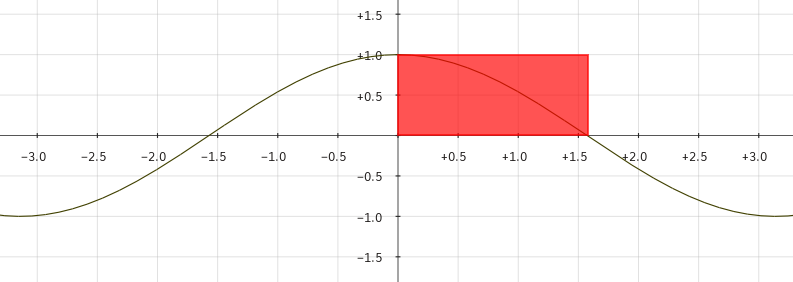
\includegraphics[width=0.8\textwidth]{img/coseno.png}
\caption{Comportamiento de la función $\cos$. En rojo la región que pertenece a la función de similitud}
\label{bus:img-coseno}
\end{figure}

%Para \textbf{similitud coseno} dos vectores proporcionales con la misma dirección la similitud es 1 (ya que es 0 el ángulo que se forma). Por lo que esta similitud no diferencia entre un artículo profesional y un artículo de un diario que cubre el mismo tópico. Por ejemplo si dos artículos que cubren un mismo y único tópico, pero para uno el valor del tópic Esta debilidad de la medida basada en el ángulo no interfiere en este trabajo por la segunda propiedad de los vectores del problema, porque para que dos vectores sean proporcionalmente iguales tienen que ser idénticos y en tal caso es correcto que la similitud entre ellos sea 1.

Con el objetivo de simplificar la ejecución de los algoritmos, considerando que el costo de calcular $cos()$ de los vectores es alto, se decidió realizar el cálculo de la similitud de los artículos, autores y universidades previamente a la ejecución de los algoritmos de búsquedas.

\subsection{Base de dato de atracciones turísticas}
Se utilizó una instancia de datos correspondiente a 200 atracciones turísticas de Europa, con datos relevados del sitio \textit{TripAdvisor}. De cada atracción se tiene la información del precio, del tipo (parque, museo, edificio) y de la distancia geográfica con el resto de las atracciones.

El propósito de la búsqueda es darle al usuario distintas opciones de circuitos turísticos que contienen atracciones, con los siguientes requerimientos: evitar realizar largos traslados, variedad en el tipo de atracción y que el costo del circuito no supere el presupuesto del turista. Por lo tanto el modelo de la búsqueda quedó diseñado de la siguiente manera: \label{busqueda:atracciones}

\begin{itemize}
	\item \textbf{Similitud}: La inversa de la distancia entre las atracciones. 
	\item \textbf{Costo}: Precio de la atracción. 
	\item \textbf{Presupuesto}: Presupuesto del turista. 
	\item \textbf{Complementariedad}: Tipo de atracción.
\end{itemize}

\section{Resultados}\label{sect:resultados}

En esta sección se analizarán los resultados computacionales comparando la calidad de las soluciones obtenidas por los algoritmos discutidos en \autoref{chap:nuevas-propuestas}, sobre las bases de datos de \autoref{sect:busquedas}. Con el objetivo de evaluar las propuestas algorítmicas, se consideraron los siguientes métodos.

\begin{itemize}
\item{$alg1$} PAC(C-HAC / selección simple)
\item{$alg2$} PAC(BOBO-10 / selección simple)
\item{$alg3$} PAC(BOBO-10 / selección proporcional)
\item{$alg4$} PAC(BOBO-10 / selección proporcional) + tabú
\item{$alg5$} PAC(Intra-Inter C-HAC / selección proporcional)
\item{$alg6$} PAC(Intra-Inter C-HAC / selección proporcional) + tabú
\item{$alg7$} Construcción golosa
\item{$alg8$} Construcción golosa + tabú
\end{itemize}

Tanto $alg1$ como $alg2$ corresponden a las metodologías propuestas en \cite{journals/tkde/Amer-YahiaBCFMZ14}. Los demás algoritmos involucran las mejoras propuestas en este trabajo. En \texttt{PAC}, la búsqueda tabú \texttt{Inter-Paquete} se realiza al finalizar la etapa de producción y la \texttt{Intra-Paquete} luego de la selección. En la \texttt{Búsqueda Golosa} se intenta mejorar la solución obtenida mediante la búsqueda tabú \texttt{Intra-Paquete}. Cabe señalar que no se tienen en consideración BOBO-Ex y CAP, ya que para el tamaño de la instancia los tiempos de ejecución de esos algoritmos resultaron prohibitivos. A partir de una experimentación preliminar con BOBO para valores $c=1, 5$ y $10$, resultó $c=10$ la opción más competitiva. Para la búsquedas tabú se definió que la cantidad de iteraciones de permanencia de un elemento en la lista tabú sea el promedio de elementos que tiene un paquete en la solución inicial.

Para realizar una comparación entre la calidad de las soluciones obtenidas por los diferentes algoritmos, se ha evaluado para los $\gamma \in \left\{0,1; 0,3; 0,4; 0,5; 0,6; 0,7; 0,8; 0,9\right\}$ el porcentaje de deterioro de cada solución respecto de la mejor solución obtenida por alguno de los ocho algoritmos.

En el caso de la búsqueda de artículos, que es el escenario que contiene la mayor cantidad de objetos, los tiempos de ejecución para los algoritmos C-HAC ($alg1$, $algo5$ y $alg6$), BOBO ($alg2$, $alg3$ y $alg4$) y los golosos ($alg7$ y $alg8$) son del orden de los 5, 2 y 6 minutos respectivamente. Los incrementos de tiempo debido a la ejecución de las metaheurísticas de mejora son despreciables, están entre los 5 y 7 segundos. Por lo cual no se considera que el tiempo sea un factor que valga la pena analizar.

\subsection{Análisis de los resultados obtenidos de la base de datos de artículos}
Para comprender el comportamiento de los resultados de las búsquedas se diseñaron dos tipos de gráficos que permiten visualizar la cohesión de los paquetes y la dispersión entre ellos. De esta forma se podrá analizar la calidad del resultado obtenido, más allá del valor de la función objetivo.

Los gráficos del estilo de la figura \ref{res:img-explain-bars} permiten analizar la distribución de los tópicos de una solución a nivel de paquete y de la relación con otros. Las filas corresponden a los 10 paquetes obtenidos y las columnas a los 37 tópicos considerados. El tamaño del círculo representa la proporción del tópico en el perfil del artículo y el color hace referencia al paquete al cual el artículo pertenece. Por lo tanto, dos artículos tendrán gran similitud cuando los patrones de sus círculos coincidan, tanto en tamaño como en distribución. Si para un paquete la distribución entre los tópicos y el tamaño de los círculos es similar entre sus artículos se puede deducir que este paquete es cohesivo (tiene buen valor intra). Por otro lado, si los patrones de los círculos de los dos artículos más similares entre distintos paquetes no coinciden, esto indica que el resultado es diverso.
\begin{figure}[H]
  \centering
    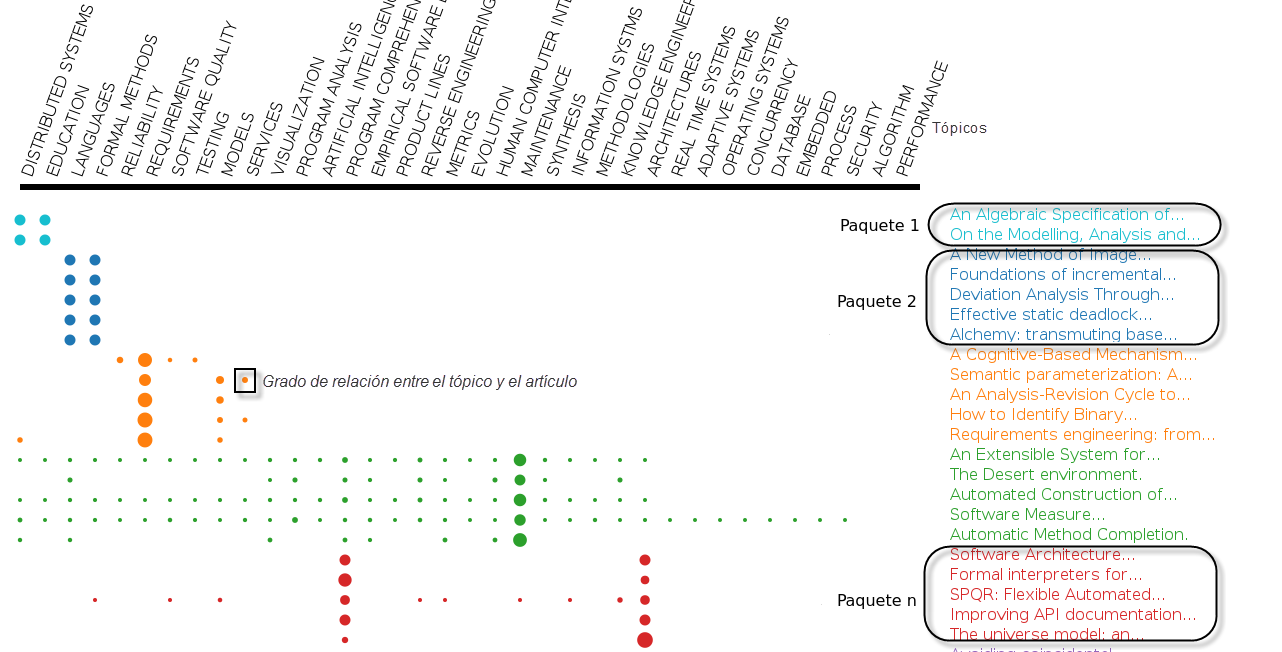
\includegraphics[width=1\textwidth]{img/explain-bars.png}
  \caption{}
  \label{res:img-explain-bars}
\end{figure}

Los gráficos de tipo burbuja de la figura \ref{res:img-explain-bubbles} son útiles para concluir el nivel de acoplamiento entre los paquetes de una solución, observando la relación entre los tópicos y los paquetes. Cada burbuja representa un tópico y cada círculo dentro de esa burbuja es un artículo. El tamaño del circulo es la proporción del artículo con el tópico y el color es el paquete al que pertenece. Entonces, si las burbujas contienen círculos de tamaños parecidos de más de un color se puede decir que ese resultado no es muy diverso. Por otro lado, mientras que el color de los círculos de las burbujas sea más homogéneo el resultado será más diverso. En cuanto a la cohesión de los paquetes, es más cohesivo cuando el tamaño de cada círculo dentro de las burbujas es similar (para el mismo color) y cada una de ellas contiene la misma cantidad, o ninguno, de círculos del mismo color.

\begin{figure}[H]
  \centering
    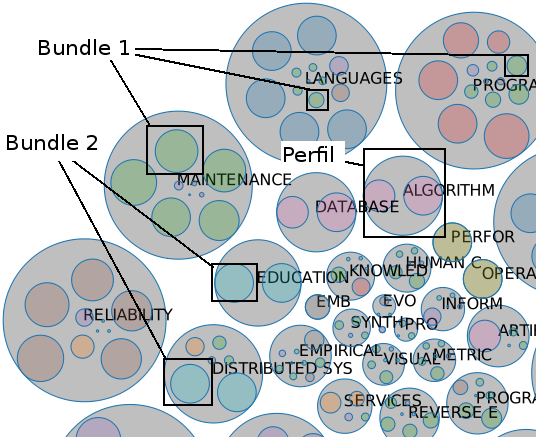
\includegraphics[width=0.5\textwidth]{img/explain-bubbles.png}
  \caption{}
  \label{res:img-explain-bubbles}
\end{figure}

\subsubsection{Búsqueda de artículos}
Para la búsqueda de artículos con tópicos similares en la tabla \ref{tabla:comp1} se observa los porcentajes de deterioro de cada solución respecto de la mejor solución obtenida por alguno de los ocho algoritmos. Una primera observación es que los algoritmos  Intra-Inter C-HAC reflejan el efecto buscado: a menores valores de $\gamma$ donde el valor inter tiene mayor peso, se obtienen mejores soluciones. Es decir, haber considerado en el proceso de generación de paquetes la función Intra-Inter benefició a la calidad de las soluciones obtenidas. Los algoritmos BOBO, no obtuvieron soluciones de la calidad de los algoritmos C-HAC y el proceso de selección proporcional no logró una mejora consistente para todos los valores de $\gamma$. Las soluciones obtenidas con el algoritmo de construcción golosa, no alcanzaron a mejorar las soluciones de C-HAC pero fueron ampliamente mejores que las de BOBO. En promedio el porcentaje de deterioro de BOBO fue de un $50\%$ mientras que el goloso fue de un $12\%$. 

Cabe resaltar el muy buen rendimiento de la búsqueda tabú, tanto en escenarios donde la solución inicial no es de buena calidad (algoritmo BOBO) así como también considerando soluciones de mejor calidad (algoritmo Intra-Inter C-HAC). En el primer caso, se obtienen porcentajes de mejora por encima del $70\%$. En el segundo caso, para varios valores de $\gamma$ la solución obtenida por la búsqueda tabú resultó ser la mejor opción y en otros con deterioros inferiores al $0.5\%$.

Si bien el algoritmo goloso no alcanzó los valores obtenidos por las soluciones generadas por C-HAC, tiene como ventaja su fácil y rápida implementación. Sus tiempos de ejecución fueron levemente mayores a los que se obtuvieron con BOBO y menores a las ejecutadas por C-HAC. Por la forma en la que fue construido siempre genera paquetes completos. Si bien la definición formal del problema no obliga a esto último, se implementó de esta manera ya que a efectos de un usuario final es más interesante obtener paquetes completos, aunque esto signifique sacrificar la búsqueda de la solución óptima.

\begin{table}[H]
\begin{center}
\begin{tabular}{|c|c|c|c|c|c|c|c|c|}
\hline
$\gamma$&$alg1$&$alg2$&$alg3$&$alg4$&$alg5$&$alg6$&$alg7$&$alg8$ \\ \hline
0.1 & -2.05 & -32.70 & -36.18 & -7.45 & -0.42 & 0.00 & -4.53 & -3.53 \\
0.2 & -2.11 & -38.06 & -41.19 & -8.23 & 0.00 & 0.00 & -4.92 & -3.85 \\
0.3 & -2.31 & -45.21 & -47.35 & -8.01 & 0.00 & 0.00 & -9.17 & -7.66 \\
0.4 & -0.14 & -49.08 & -51.22 & -15.51 & 0.00 & 0.00 & -10.40 & -9.35 \\
0.5 & 0.00 & -52.35 & -54.23 & -17.87 & -0.31 & -0.31 & -12.97 & -10.38 \\
0.6 & 0.00 & -55.16 & -56.04 & -14.43 & -0.05 & -0.05 & -14.78 & -13.69 \\
0.7 & 0.00 & -56.88 & -56.57 & -17.02 & -0.41 & -0.41 & -16.21 & -15.08 \\
0.8 & 0.00 & -57.86 & -57.86 & -16.11 & -0.56 & -0.30 & -18.10 & -17.60 \\
0.9 & 0.00 & -58.92 & -58.92 & -15.91 & -0.48 & -0.35 & -20.47 & -17.61 \\ \hline 
\end{tabular}
\caption{Comparación de calidad de soluciones entre algoritmos para la \hyperref[busqueda:articulos]{búsqueda de artículos}} 
\label{tabla:comp1}
\end{center}
\end{table}

Para comprender la semántica de las soluciones se compararon las soluciones con $\gamma = 0,1$ y $\gamma = 0,9$. En la figura \ref{res:comp1} se observa que para $\gamma = 0,1$ los tópicos (representados por burbujas) para la solución de \textit{alg 3} están presentes en varios paquetes (representados por círculos de colores). En cambio en el $alg6$ la mayoría de las burbujas contiene círculos de un solo color. De esta manera se visualiza que la solución de $alg6$ es más diversa. En $\gamma = 0,9$ el resultado obtenido con $alg3$ no se visualiza que cada burbuja contenga cinco círculos del mismo color, en cambio si sucede para la solución de $alg1$. Eso significa que los paquetes de la solución de $alg1$ son más cohesivos, ya que los cinco elementos de cada paquete tienen los mismos tópicos.

\begin{figure}[H]
	\centering
	\begin{tabular}{cc}
		\multicolumn{2}{c}{$\gamma=0.1$}\vspace{0.5cm}\\
		$alg3$ & $alg6$\\
		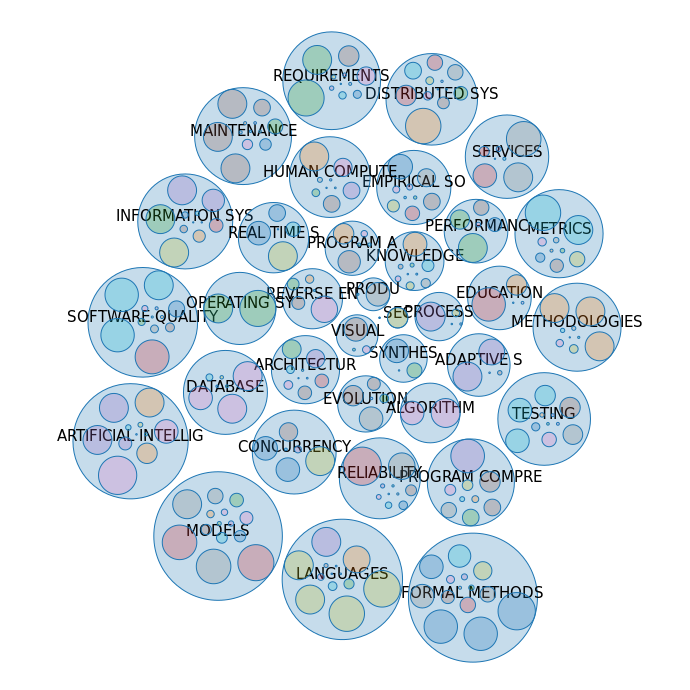
\includegraphics[width=0.45\linewidth]{img/gamma-01-burbujas-alg-3.png}&
		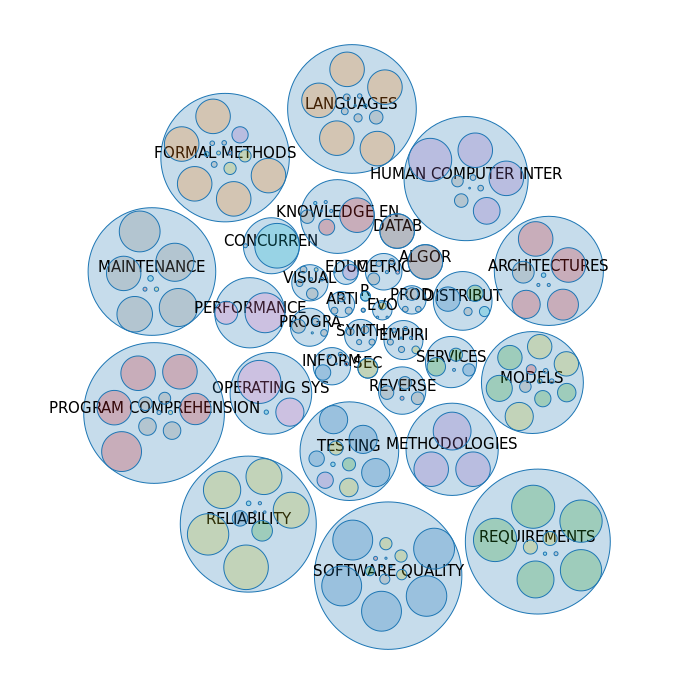
\includegraphics[width=0.45\linewidth]{img/gamma-01-burbujas-alg-6.png}\vspace{1cm}\\
		\multicolumn{2}{c}{$\gamma=0.9$}\vspace{0.5cm}\\
		$alg3$ & $alg1$\\
		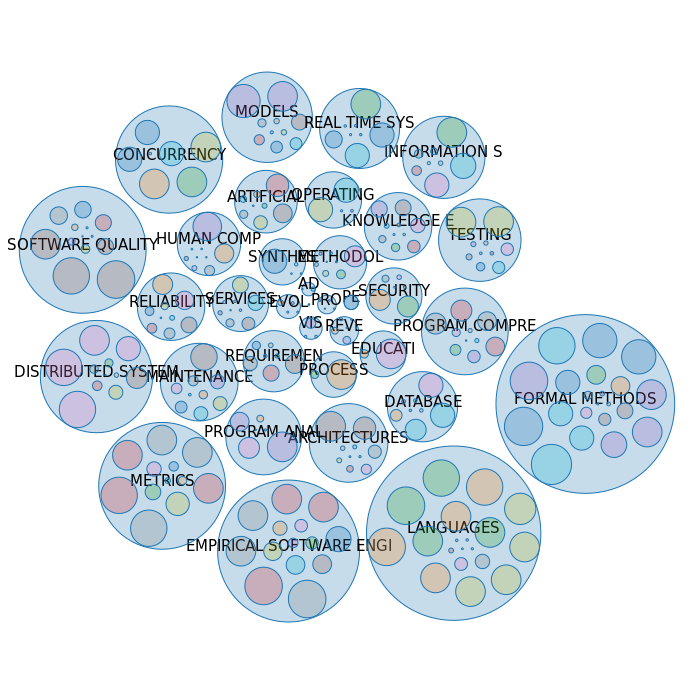
\includegraphics[width=0.45\linewidth]{img/gamma-09-burbujas-alg-3.png}&
		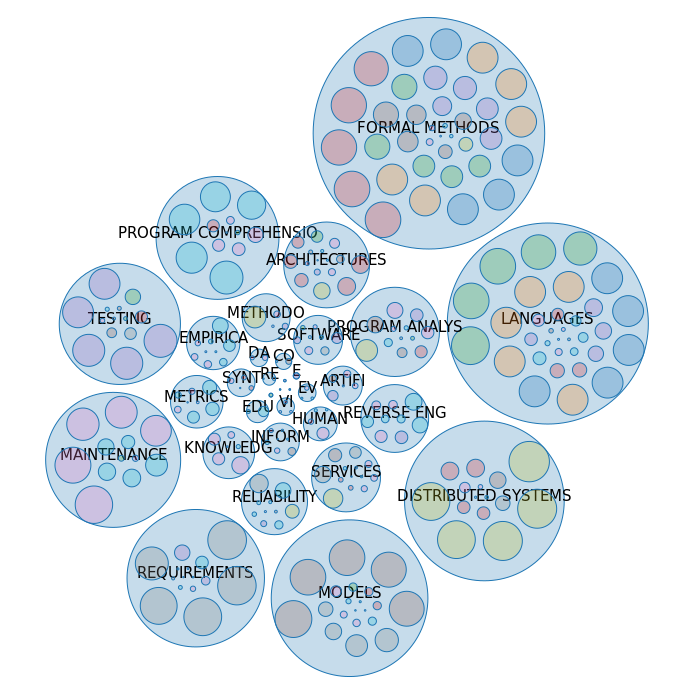
\includegraphics[width=0.45\linewidth]{img/gamma-09-burbujas-alg-1.png}\\
	\end{tabular}
	\caption{Comparación entre las soluciones con menor(izq) y mayor(der) función objetivos  para $\gamma\ =\ 0,1\ y \gamma\ =\ 0,9$}
	\label{res:comp1}
\end{figure}

La búsqueda tabú tiene su mayor impacto cuando es aplicada a la solución brindada por el algoritmo $alg3$, como puede observarse en la tabla \autoref{tabla:comp1} y en este contexto resulta una buena alternativa por su bajo costo computacional. En la Figura~\ref{res:bobo} se observa que para $\gamma=0.1$, la solución dada por el $alg3$ tiene artículos de distintos paquetes con patrones muy similares indicando un bajo valor inter-paquete. Por el contrario, luego de aplicar la búsqueda tabú los patrones de los artículos más similares entre distintos paquetes se volvieron más dispares, demostrando el aumento de la diversidad entre paquetes. Para $\gamma=0.9$, como puede observarse en la misma Figura~\ref{res:bobo}, en la solución brindada por el $alg4$ todos los paquetes tienen al menos un artículo cuyo patrón consiste en muchos círculos pequeños distribuidos en la mayoría de los tópicos en contraposición al resto de los artículos del mismo paquete con pocos círculos de gran tamaño. Demostrando un bajo valor intra-paquete. En contraposición a los paquetes obtenidos luego de aplicar la búsqueda tabú, los cuáles son mucho más cohesivos. La última afirmación puede observarse en los círculos de los artículos dentro de un mismo paquete, quienes siguen patrones mucho más parecidos. Se puede afirmar que la búsqueda tabú es capaz de mejorar las características de la solución en función del parámetro $\gamma$.

\begin{figure}[H]
	\centering
	\begin{tabular}{cc}
		$alg3$ & $alg4$\vspace{0.5cm}\\
		\multicolumn{2}{c}{$\gamma=0.1$}\\
		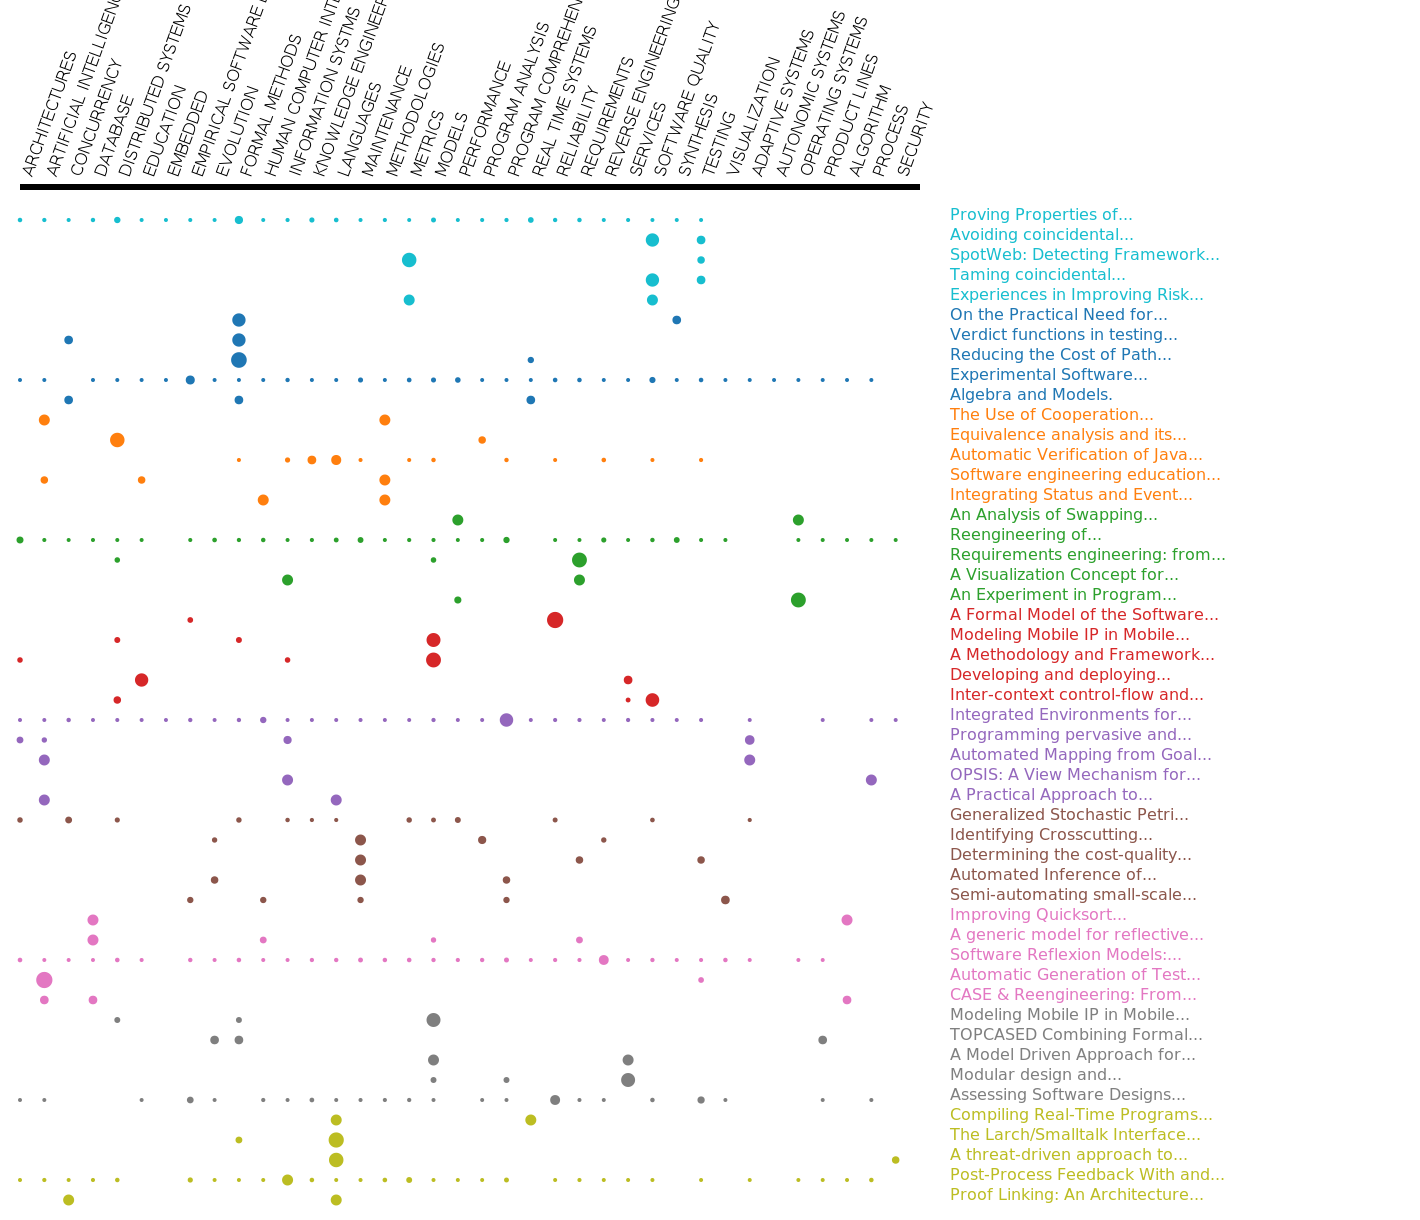
\includegraphics[width=0.45\linewidth]{img/gamma-01-alg-3.png}&
		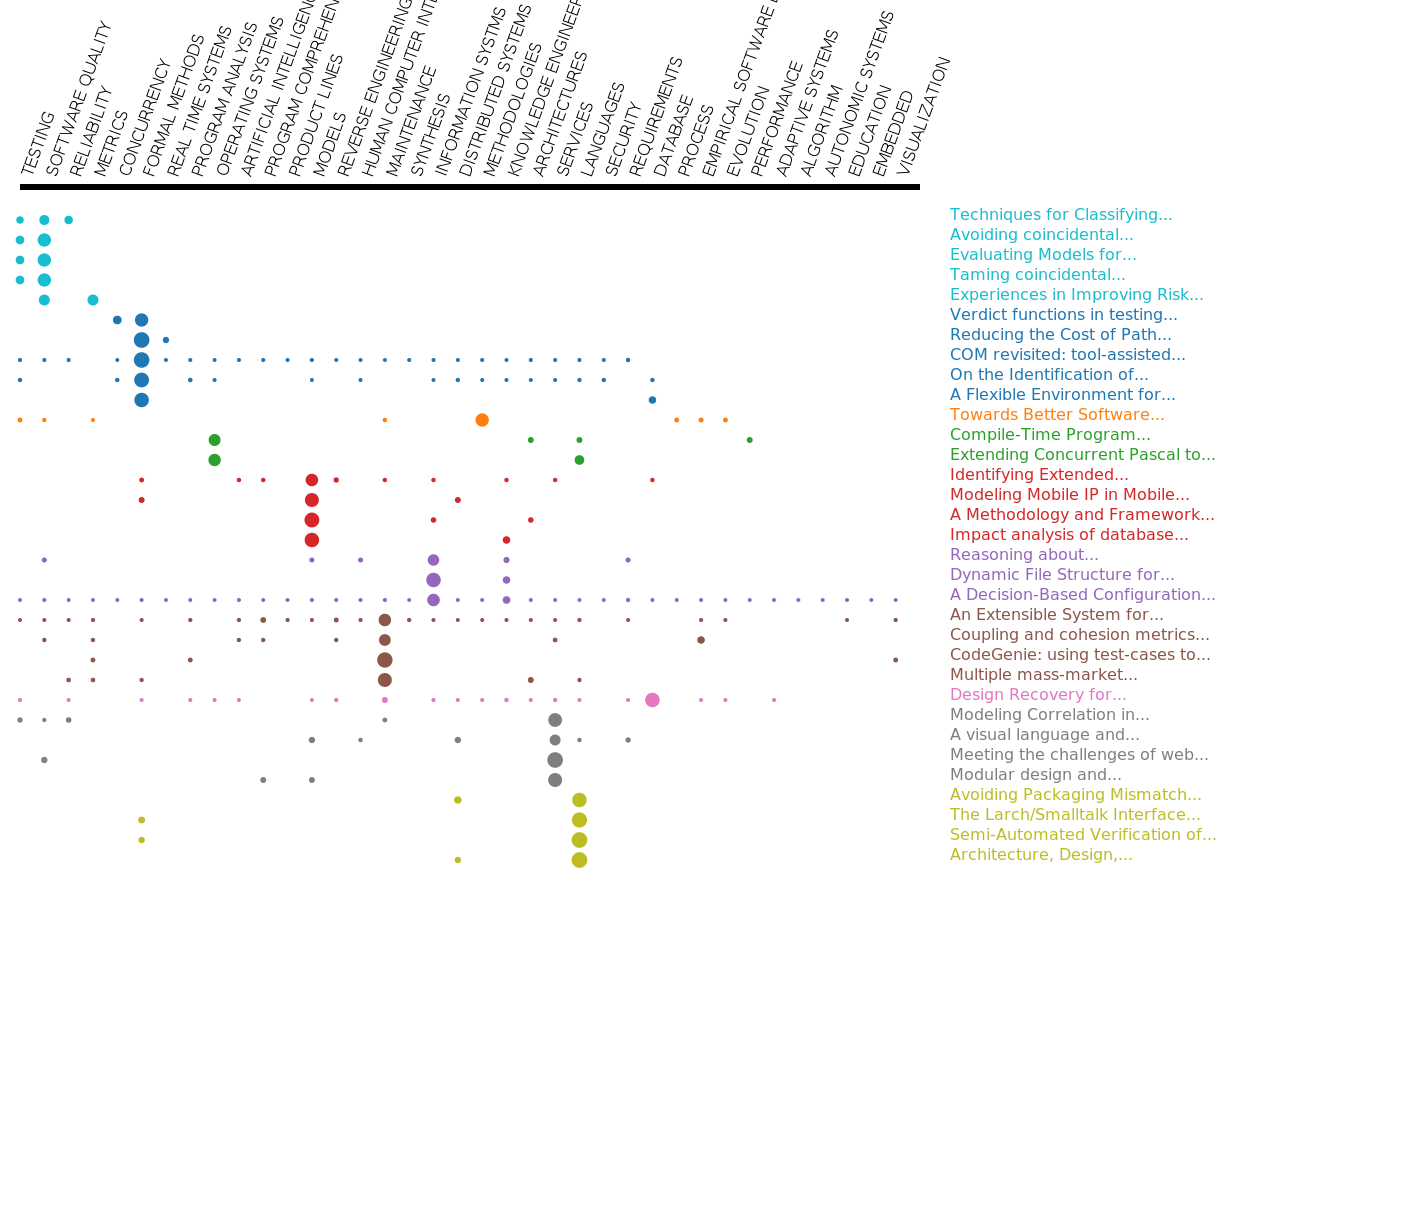
\includegraphics[width=0.45\linewidth]{img/gamma-01-alg-4.png}\vspace{1cm}\\
		\multicolumn{2}{c}{$\gamma=0.9$}\\
		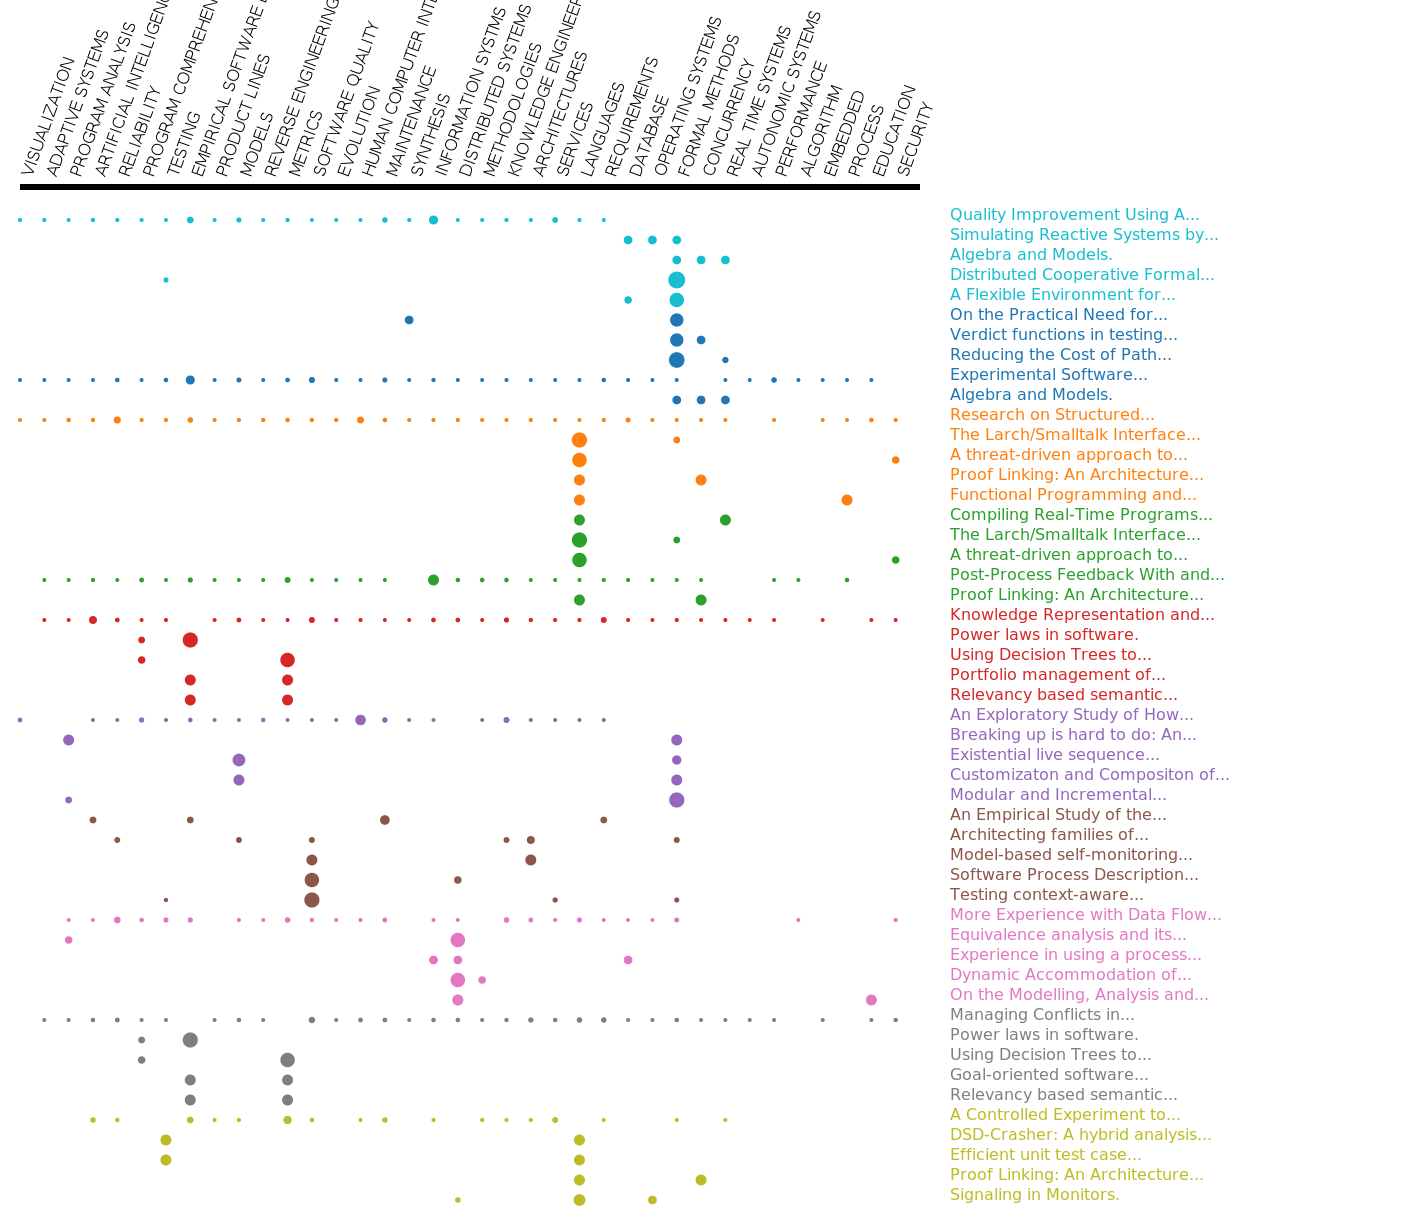
\includegraphics[width=0.45\linewidth]{img/gamma-09-alg-3.png}&
		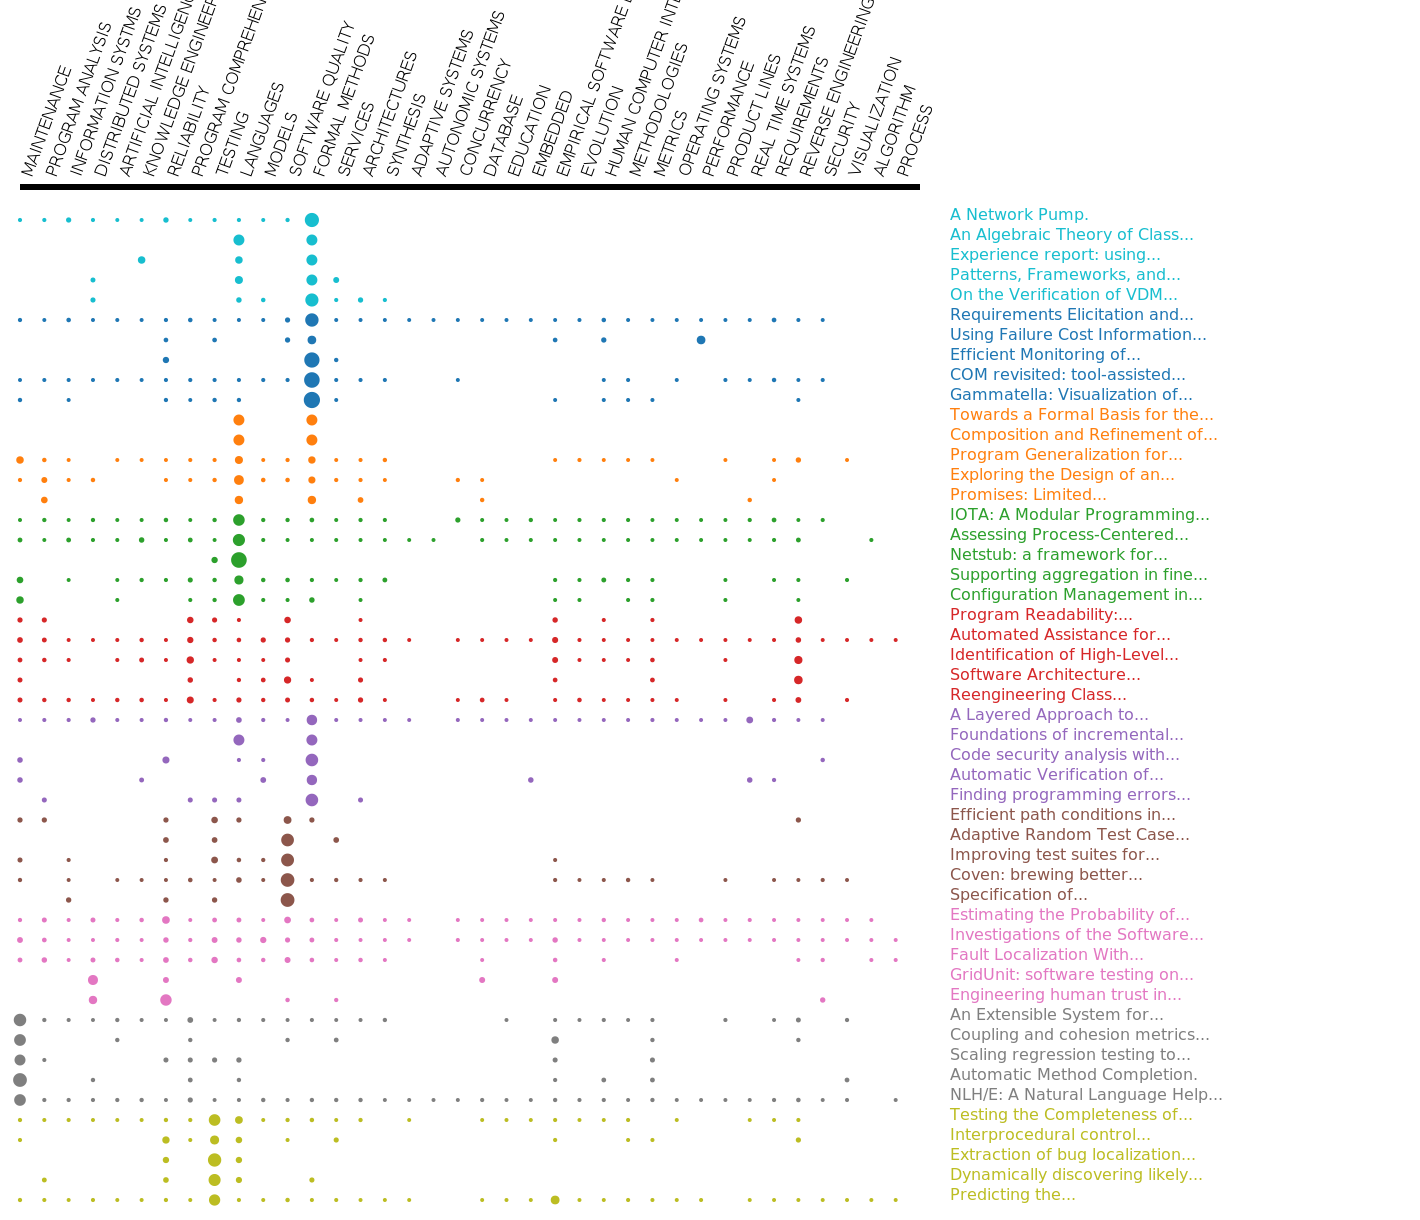
\includegraphics[width=0.45\linewidth]{img/gamma-09-alg-4.png}\\
	\end{tabular}
	\caption{Comparación de soluciones para BOBO-10 con y sin heurística de mejoramiento}
	\label{res:bobo}
\end{figure}

La decisión acerca del valor de $\gamma$ para priorizar un objetivo sobre el otro es realizada por el usuario. Una curva de frontera eficiente podría ayudar para examinar el balance (trade-off) entre los dos objetivos. La intención es que el usuario pueda analizar si una mejora significativa en el valor intra-paquete implica una degradación sustancial en el valor inter-paquetes y viceversa. Para ilustrar este análisis en la Figura \ref{res:inter_intra} se comparan las soluciones obtenidas por los algoritmos $alg1$ y $alg5$ variando en pasos de $0,1$. Una primera evaluación muestra que la mayoría de las soluciones provistas por ambos algoritmos son no dominadas, es decir ninguna solución es mejor en ambos objetivos que cualquier otra solución.

El algoritmo $C-HAC$ de \cite{journals/tkde/Amer-YahiaBCFMZ14} ($alg1$) utiliza la función $Score$ para decidir el par de {\em clusters} a unir en la etapa de producción de paquetes y en la selección simple en la segunda fase. Estos dos criterios omiten la diversidad de los paquetes. De acuerdo a los resultados de la tabla \ref{tabla:comp1}, se pudo concluir que haber considerado la función Intra-Inter y la selección proporcional benefició la calidad de las soluciones cuando la misma es medida a partir de la función objetivo $w(S)$. Con el fin de evaluar que el $alg5$ es capaz de captar efectivamente la diversidad en la solución, se analizaron las soluciones para $\gamma=0.5$. En este caso el $alg1$ obtuvo un valor de $intra=93,82$ y de $inter=35,49$, mientras que el $alg5$ logró valores de $intra=92,94$ y de $inter=35,96$. A pesar de que la solución de $alg1$ es levemente superior, la solución del $alg5$ aumentó el valor $inter$ el $1,32\%$ con un deterioro del valor $intra$ del $0,93\%$. Observando la Figura~\ref{res:inter_intra} se puede ver que la cohesión intra-paquete de ambas soluciones es equivalente. Sin embargo, la diversidad en la segunda solución es mayor, ya que los patrones entre los artículos más similares de distintos paquetes son más heterogéneos. 

En la misma figura se compara las soluciones obtenidas por los algoritmos $alg2$ y el goloso $alg7$. En promedio supera a las soluciones provistas por $alg2$ en $76\%$. De la comparación, se destaca que el valor de $\gamma$ impacta más en las soluciones de $alg2$.  

\begin{figure}[H]
	\centering
	\begin{tabular}{cc}
			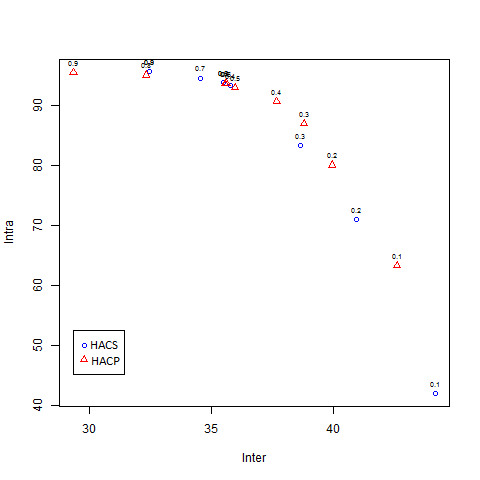
\includegraphics[width=0.45\linewidth]{img/alg1_vs_alg5.png}&
			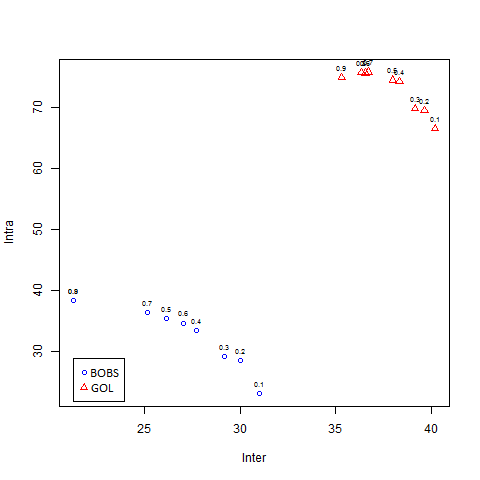
\includegraphics[width=0.45\linewidth]{img/alg2_vs_alg7.png}\\
			$alg1$ vs $alg5$ & $alg2$ vs $alg7$\\
	\end{tabular}
	\caption{Trade-off entre objetivos para los distinos valores de $\gamma$}
	\label{res:inter_intra}
\end{figure}

\subsubsection{Búsqueda de autores}
En la tabla \ref{tabla:comp2} se muestran los porcentajes de deterioro de cada solución con respecto a la mejor solución obtenida para la búsqueda de ``autores que escribieron artículos de tópicos similares que están afiliados a distintas universidades''. Se observa que en este caso, a diferencia de la búsqueda de artículos, el algoritmo tabú halló en todos los casos la mejor solución. Con la particularidad que el algoritmo goloso tuvo muy poco deterioro con respecto a la mejor solución, alcanzando en algunos casos el mismo valor de función objetivo.

Los algoritmos jerárquicos $C-HAC$ e $Inter-Intra C-HAC$ siguen demostrando que obtienen las mejores soluciones en comparación a $BOBO$, sobre todo $alg6$ que contiene la búsqueda tabú. Éstas búsquedas vuelven a indicar que las soluciones pueden ser mejoradas en porcentajes muy significativos. Como ocurrió en el caso del algoritmo $alg3$, mejorando las soluciones en un promedio cercano al $30\%$ y también para $alg5$ y $alg7$ que en todos los casos mejoraron sus valores iniciales. Con respecto a la estrategia de selección proporcional aplicada al algoritmo $BOBO$ no se observaron mejoras, aunque las soluciones obtenidas fueron cercanas en términos de función objetivo. 

\begin{table}[H]
\begin{center}
\begin{tabular}{|c|c|c|c|c|c|c|c|c|}
\hline
$\gamma$&$alg1$&$alg2$&$alg3$&$alg4$&$alg5$&$alg6$&$alg7$&$alg8$ \\ \hline
0.1 & -0.33 & -21.59 & -26.05 & -1.74 & -0.13 & 0.00 & -0.61 & 0.00 \\
0.2 & -0.63 & -27.46 & -29.71 & -0.52 & -0.36 & 0.00 & -1.10 & -0.25 \\
0.3 & -0.44 & -30.57 & -32.47 & -0.20 & -0.53 & 0.00 & -1.50 & -0.34 \\
0.4 & -0.25 & -32.63 & -34.29 & -0.32 & -0.25 & 0.00 & -1.88 & -0.73 \\
0.5 & -0.22 & -34.42 & -35.84 & -0.04 & 0.00 & 0.00 & -2.15 & -0.79 \\
0.6 & -0.18 & -35.86 & -37.05 & -2.01 & 0.00 & 0.00 & -2.45 & -1.39 \\
0.7 & 0.00 & -37.10 & -37.93 & -1.71 & -0.12 & 0.00 & -2.59 & -0.96 \\ 
0.8 & 0.00 & -38.19 & -38.70 & -1.44 & -0.08 & 0.00 & -2.72 & -1.20 \\
0.9 & -0.03 & -39.15 & -39.38 & -1.21 & -0.10 & 0.00 & -3.35 & -1.72 \\ \hline 
\end{tabular}
\caption{Comparación de calidad de soluciones entre algoritmos para la \hyperref[busqueda:autores]{búsqueda de autores}} 
\label{tabla:comp2}
\end{center}
\end{table}

Para analizar el trade-off entre la parte inter y la intra en la figura \ref{res:aut_alg1_vs_alg5_vs_alg7} del lado izquierdo se muestra los valores inter e intra de las soluciones obtenidas por los algoritmos $alg1$, $alg2$, $alg5$ y $alg7$ para todos los $\gamma$. Puede apreciarse, como es de esperar, que los valores del $alg2$ son significativamente inferiores al resto de los algoritmos. En cambio los valores de $alg1$, $alg5$ y $alg7$ se concentran en una región reducida, ya que sus soluciones fueron muy similares respecto al valor de la función objetivo.

A la derecha de la figura \ref{res:aut_alg1_vs_alg5_vs_alg7} se encuentran los valores inter e intra de los algoritmos $alg1$ y $alg5$. Puede verse como los valores de las soluciones obtenidas con $alg5$ no están dominadas por la parte inter y si más concentradas en la parte intra, a diferencia de los que ocurre con $alg1$.

\begin{figure}[H]
	\centering
	\begin{tabular}{cc}
			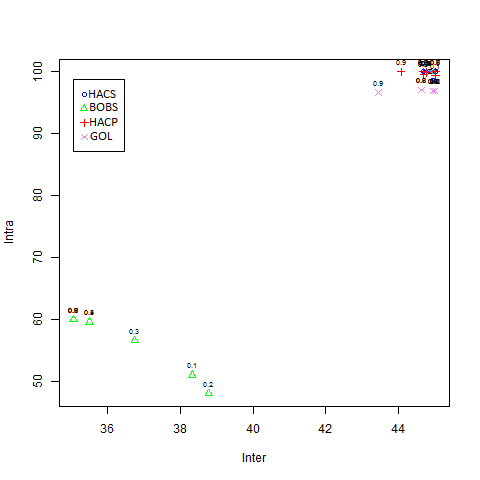
\includegraphics[width=0.45\linewidth]{img/aut-alg1-alg2-alg5-alg7.png}&
			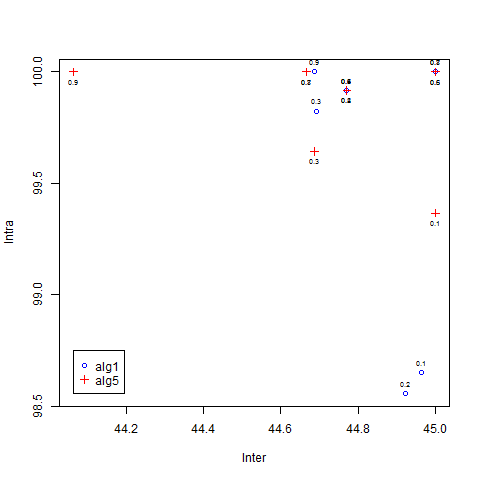
\includegraphics[width=0.45\linewidth]{img/aut-alg1-alg5.png}\\
	\end{tabular}
	\caption{}
	\label{res:aut_alg1_vs_alg5_vs_alg7}
\end{figure}


En la figura \ref{res:aut-alg-6} de la solución generada por el algoritmo $alg6$ para $\gamma = 0.1$, se tienen las siguientes observaciones:
\begin{enumerate}
	\item Todos los paquetes contienen autores que pertenecen a los mismos tópicos. 
	\item No existe un tópico que esté presente en más de un paquete.
	\item Todos los paquetes utilizan el máximo del presupuesto.
\end{enumerate}
Por (1) y (2) la calidad intra e inter paquete es máxima respectivamente. Con (3) se cumple que la solución obtenida es la de máxima calidad para todo $\gamma$. Para todas las búsquedas realizadas, las soluciones que se obtuvieron cumplían con las observaciones mencionadas.

\begin{figure}[H]
  \centering
    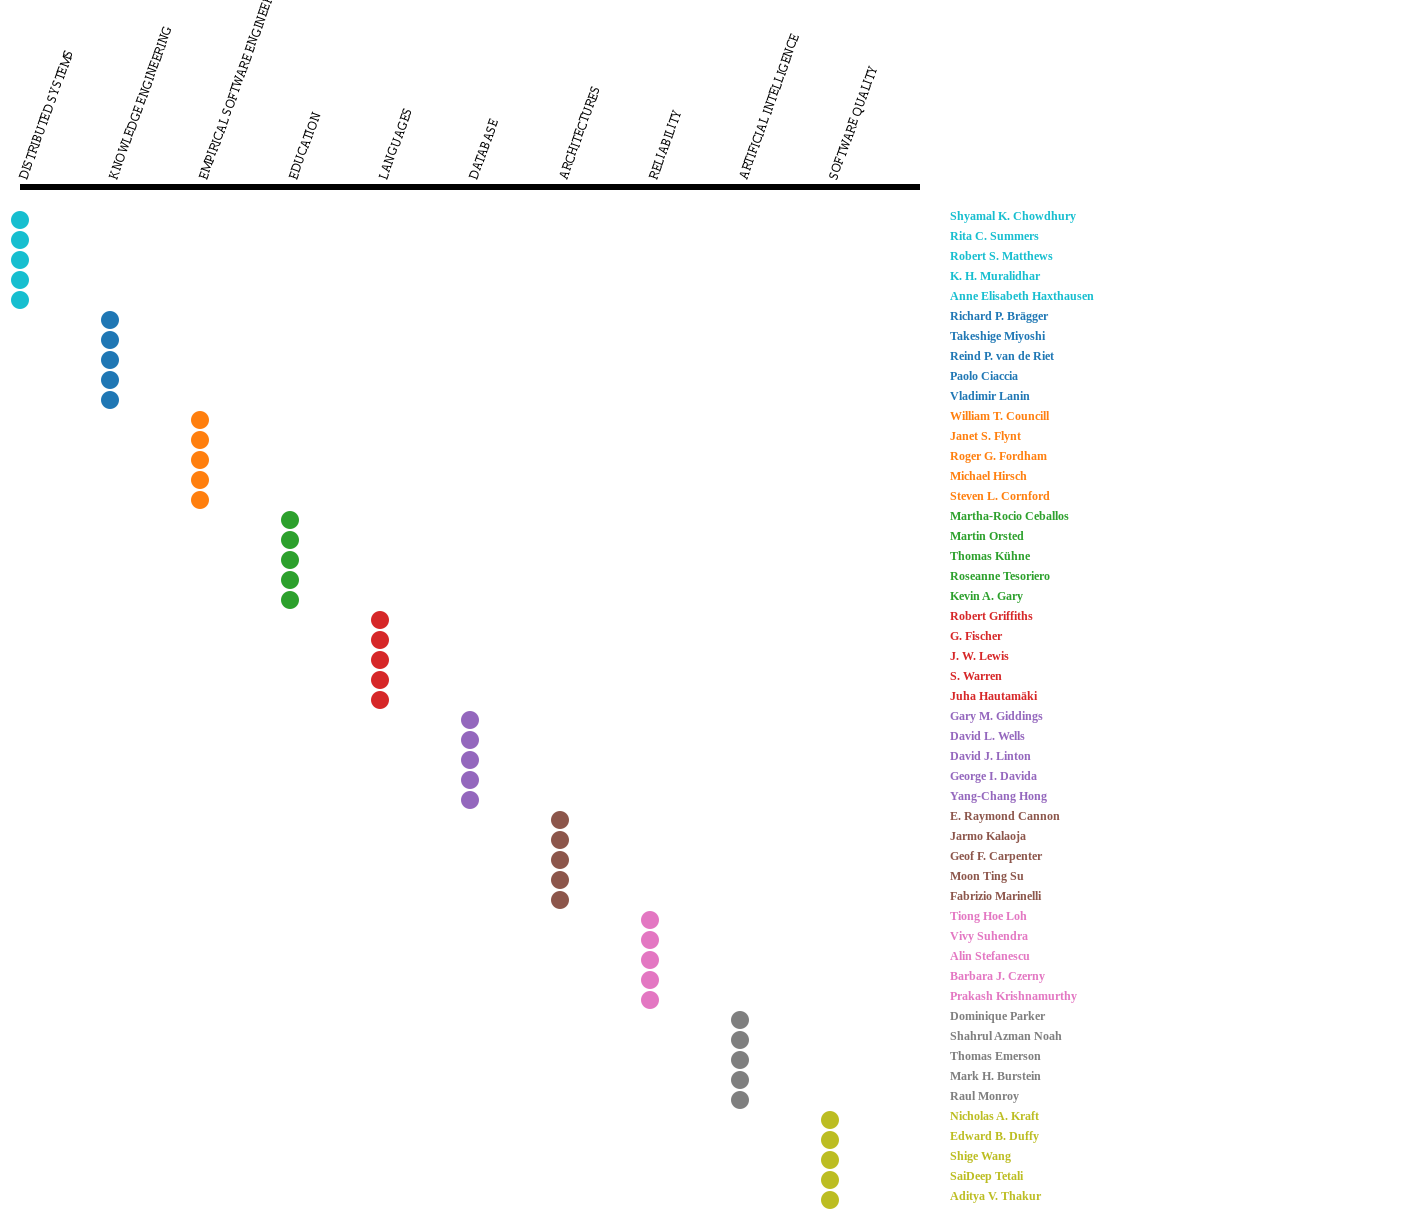
\includegraphics[width=1\textwidth]{img/aut-alg-6.png}
  \caption{}
  \label{res:aut-alg-6}
\end{figure}



\subsubsection{Búsqueda de universidades}
En este escenario lo que más se destaca de la tabla \ref{tabla:comp3} es el comportamiento del algoritmo $alg1$ que generó una mejor solución para los valores de $\gamma\ =\ 0.1$ y $\gamma\ =\ 0.2$ con respecto al algoritmo $alg6$. En el resto de las soluciones obtenidas (de $alg1$ y $alg6$) se aprecia un deterioro cada vez más significativo a medida que crece el valor del $\gamma$.

Por otro lado la función objetivo de las soluciones provista por los algoritmos $alg2$, $alg3$ y $alg7$ se encuentran muy alejadas de las soluciones provistas por los jerárquicos. En el caso del algoritmo goloso $alg7$ las soluciones mejoran con respecto a los algoritmos $alg2$ y $alg3$ cuando el valor de $\gamma$ disminuye.

Al igual que en el resto, la búsqueda tabú mejoró las soluciones iniciales del $BOBO$ y del algoritmo goloso considerablemente. Se destaca que para las soluciones jerárquicas la búsqueda tabú siempre mejora la solución inicial sin importar que tan buena sea.
\begin{table}[H]
\begin{center}
\begin{tabular}{|c|c|c|c|c|c|c|c|c|}
\hline
$\gamma$&$alg1$&$alg2$&$alg3$&$alg4$&$alg5$&$alg6$&$alg7$&$alg8$ \\ \hline
0.1 & 0.00 & -30.89 & -31.26 & -15.05 & -1.39 & -1.33 & -10.97 & -9.73 \\
0.2 & 0.00 & -40.35 & -40.16 & -22.09 & -1.72 & -1.07 & -22.83 & -20.42 \\
0.3 & -2.22 & -50.85 & -49.98 & -27.01 & -2.37 & 0.00 & -36.06 & -28.55 \\
0.4 & -5.72 & -60.65 & -58.96 & -33.76 & -1.36 & 0.00 & -48.44 & -30.38 \\
0.5 & -8.59 & -69.76 & -67.66 & -31.46 & -1.92 & 0.00 & -60.18 & -34.32 \\
0.6 & -12.09 & -77.50 & -74.71 & -33.85 & -2.53 & 0.00 & -70.16 & -35.80 \\
0.7 & -12.59 & -82.97 & -80.09 & -31.52 & 0.00 & 0.00 & -78.04 & -29.36 \\
0.8 & -15.52 & -88.12 & -84.93 & -32.90 & 0.00 & 0.00 & -85.63 & -36.34 \\
0.9 & -17.46 & -88.10 & -87.79 & -31.16 & 0.00 & 0.00 & -92.13 & -28.26 \\
 \hline 
\end{tabular}
\caption{Comparación de calidad de soluciones entre algoritmos para la \hyperref[busqueda:universidades]{búsqueda de universidades}} 
\label{tabla:comp3}
\end{center}
\end{table}

\subsection{Análisis de los resultados obtenidos de la base de datos de atracciones turísticas}\label{res:busAtracciones}
En las búsquedas realizadas sobre la base de datos de atracciones turísticas las soluciones obtenidas a partir de las modificaciones propuestas en este trabajo de los algoritmos PAC, como puede observarse en la tabla \ref{tabla:comp4}, mejoran a los originales en todos los casos. Es para destacar que en este escenario el algoritmo goloso supera a $alg1$. La búsqueda tabú consiguió mejores resultados para los algoritmos PAC. Por otro lado en el algoritmo goloso, en contraste a lo sucedido en las demás consultas, la heurística de búsqueda no obtuvo mejores soluciones.

\begin{table}[H]
\begin{center}
\begin{tabular}{|c|c|c|c|c|c|c|c|c|}
\hline
$\gamma$&$alg1$&$alg2$&$alg3$&$alg4$&$alg5$&$alg6$&$alg7$&$alg8$ \\ \hline
0.1 & -6.49 & -22.89 & -22.30 & -9.99 & -0.05 & 0.00 & -0.52 & -0.52 \\
0.2 & -13.50 & -27.60 & -26.57 & -16.51 & -0.09 & 0.00 & -1.09 & -1.09 \\
0.3 & -21.10 & -32.76 & -29.73 & -20.58 & -0.15 & 0.00 & -1.70 & -1.70 \\
0.4 & -29.38 & -36.68 & -33.51 & -25.10 & -0.20 & 0.00 & -2.37 & -2.37 \\
0.5 & -38.43 & -42.05 & -38.44 & -30.94 & -0.27 & 0.00 & -3.10 & -3.10 \\
0.6 & -48.35 & -47.73 & -43.86 & -34.75 & -0.34 & 0.00 & -3.90 & -3.90 \\
0.7 & -59.29 & -51.47 & -50.54 & -43.46 & -0.41 & 0.00 & -4.78 & -4.78 \\
0.8 & -71.36 & -57.07 & -56.14 & -45.61 & 0.00 & 0.00 & -5.62 & -5.62 \\
0.9 & -84.97 & -60.59 & -59.81 & -44.04 & 0.00 & 0.00 & -7.33 & -7.33 \\
\hline 
\end{tabular}
\caption{Comparación de calidad de soluciones entre algoritmos para la \hyperref[busqueda:atracciones]{búsqueda de atracciones turísticas}}
\label{tabla:comp4}
\end{center}
\end{table}

\subsection{Análisis general de los resultados obtenidos}
Se obtuvieron mejores resultados en términos de los valores de la función objetivo, así como en la sensibilidad al criterio de valorización de cada objetivo sin perjuicio en el tiempo de ejecución. En el caso de los algoritmos $PAC$ usando generación de paquetes mediante las técnicas $BOBO$ y aplicando la búsqueda tabú el resultado mejoró considerablemente, como puede verse en \autoref{tabla:comp1} y \autoref{tabla:comp2}.

Se observó que las soluciones obtenidas utilizando el algoritmo goloso fueron mejores en comparación a las generadas por la metodología $PAC$, solo cuando en la etapa de producción se utilizó la estrategia $BOBO$. Por el contrario, la producción jerárquica derivó en la obtención final de mejores paquetes. Si bien la técnica de las implementaciones de $BOBO$ son golosas, éstas solo hacen hincapié en los valores intra de la función objetivo. Mientras qué la nueva propuesta lo hace sobre la totalidad de la función objetivo. 

Para la estrategia PAC las implementaciones de BOBO fueron en todos los casos las más rápidas, resultando ser las ideales para instancias de tamaño muy grandes. La solución obtenida mejorá considerablemente si se le aplica la búsqueda tabú. En las pruebas realizadas con HAC con un universo de elementos menor a los 10000 se cuadruplican o quintuplican los tiempos de ejecución debido a su complejidad ($\mathcal{O}(N^{2}\log n)$). Sin embargo en instancias más chicas como las atracciones turísticas los tiempos fueron muy cercanos entre ellos.

Las soluciones obtenidas usando \texttt{Efficient-HAC} y búsquedas golosas para valores de $\gamma$ menores a $0.5$ fueron \textquotedblleft similarmente buenas\textquotedblright , dado que los resultados en términos de función objetivo fueron cercanos. En cambio para $\gamma$ más cercanos a uno se observó que el valor de la función objetivo de las soluciones HAC resultaron significativamente mayores. En todos los casos se identificó que las relaciones inter-paquetes son mejores en las soluciones del algoritmo goloso, logrando soluciones más interdependientes.

Al comparar \texttt{BOBO-10} y \texttt{BOBO-160} usando la selección simple se observa que la diferencia entre los valores de la función objetivo de cada solución aumenta a medida que $\gamma$ se acerca a $1$. Se supone que esto se debe a la estrategia \texttt{produce and choose}. El objetivo de la primera etapa es producir paquetes con máximo valor de similitud. En el caso de que se requiera una solución con mayor separación entre paquetes, al haber producido menos cantidad de paquetes existen menos posibilidades para generar una solución más dispersa. Un mismo análisis se podría hacer si se compara \texttt{BOBO-10} y \texttt{HAC}.

Comparando los resultados obtenidos al realizar la selección de a un candidato contra la selección de a pares se obtuvo que para \texttt{BOBO-160} y \texttt{HAC} los tiempos aumentaron a $40$ minutos y para \texttt{BOBO-10} a $2$ minutos. En cuanto al valor de la función objetivo el único beneficiado fue \texttt{BOBO-10} ya que para \texttt{HAC} empeoró y para \texttt{BOBO-160} el aumento fue muy pequeño en comparación al incremento de tiempo.
\chapter{Conclusiones}
\label{chap:conclusiones}
\section{Comparaciones entre los diferentes algoritmos}\label{conc:compDifAlgo}
\subsection{Papers}
Con los resultados obtenidos podemos hacer dos tipos de análisis y comparaciones, la primera y más 
clara es comparar entre los algoritmos \texttt{SingleHAC} y \texttt{EfficientHAC}, en la que 
observamos que para $\gamma$ bajos obtuvimos los mismos resultados, pero para $\gamma$ altos a 
partir de $0.7$ obtuvimos soluciones diferentes las cuáles tenían un valor con respecto a la 
función objetivo prácticamente iguales pero se obtuvieron mejores relaciones interbundles.\\
La otra comparación que surge es entre \texttt{EfficientHAC} y \texttt{Greedy} en el que se observa 
que para $\gamma$ las soluciones obtenidas son \textquotedblleft similarmente 
buenas\textquotedblright , dado que sus valores en términos de función objetivo están cercanos, 
pero a la vez observamos que la relación interbundles es mejor las soluciones de la implementación 
\texttt{Greedy}. En cambio para $\gamma$ altos, el valor de la función objetivo en la 
implementación \texttt{EfficientHAC} fue muy superior pero la relación interbundles en el algoritmo 
\texttt{Greedy} se ve que fue mejor, logrando soluciones mas interdependientes.

\section{Valores cercanos al óptimo}
Dada la función que se está intentando maximizar $$\displaystyle\sum_{1 \leq i \leq k} 
\displaystyle\sum_{u,v \in S_{i}} \gamma s(u,v)\ 
+\ \displaystyle\sum_{1 \leq i \leq j \leq k} (1-\gamma) (1 - \displaystyle\max_{u \in S_{1}, v 
\in S_{j}} s(u,v))$$ podemos hacer suposiciones para ver que tan lejos o cerca están de algunas de 
los valores óptimos según el $\gamma$.\\
Para las siguientes cotas supongamos escenarios ideales en el cuál la soluciones contiene bundles 
donde todos sus elementos tienen una similitud máxima (igual a 1) y los bundles entre si son 
completamente diferentes, o sea, la similitud entre cada bundle es 0. Con estas hipótesis podemos 
ver que la reemplazar la función por $$\displaystyle\sum_{1 \leq i \leq k} 
\displaystyle\sum_{u,v \in S_{i}} \gamma 1\ 
+\ \displaystyle\sum_{1 \leq i \leq j \leq k} (1-\gamma) (1 - \displaystyle\max_{u \in S_{1}, v 
\in S_{j}} 0)$$ que luego se transforma en $$\displaystyle\sum_{1 \leq i \leq k} 
\displaystyle\sum_{u,v \in S_{i}} \gamma 1\ 
+\ \displaystyle\sum_{1 \leq i \leq j \leq k} (1-\gamma) 1$$ como en nuestro caso $k\ =\ 10$ y la 
cantidad de items por bundle es $5$ entonces la sumatoria se resume en $$\displaystyle\gamma\ 100\ 
+\ (1-\gamma)\ 45$$
Para los $\gamma \in (0.1, 0.3, 0.5, 0.7, 0.9)$ los resultados de la función son los siguientes:\\
\begin{table}[H]
  \centering
  \resizebox{0.5\textwidth}{!} {
    \begin{tabular}{|lc|}
    \hline
    $\gamma$ & Valor función objetivo \\
    \hline
    $0.1$  & $50.5$ \\
    $0.3$  & $61.5$ \\
    $0.5$  & $72.5$ \\
    $0.7$  & $83.5$ \\
    $0.9$  & $94.5$ \\
    \hline
    \end{tabular}
  }
    \caption {Valor óptimo de la función para cada $\gamma$}
\end{table}

En las ejecuciones del algoritmo \textbf{SingleHAC} para artículos en los $\gamma$ más altos los 
resultados de los bundles eran los mismos lo cuál se explica porque a medida que $\gamma$ aumenta se 
acerca cada vez más a la cota superior que establecimos. No sucediendo los mismo con $\gamma$ 
menores.\\
En cambio para las ejecuciones también del algoritmo \textbf{SingleHAC} pero para autores en todas 
las soluciones obtuvimos los mismos bundles y se ve reflejado porque la función objetivo para cada 
$\gamma$ es igual a la cota.

%\chapter{Apéndice}
%\section{Resultados de las ejecuciones de los algoritmos de búsqueda}
A continuación se muestra el valor de la función objetivo para cada uno de los distintos algoritmos ejecutados y el tiempo de ejecución final.
\subsection{Artículos}
\Solucion
{}
{simple, por tuplas y proporcional}
{\texttt{HAC} y \texttt{BOBO-x}, con  $x \in$ $(10, 160)$}
{$\in$ $(0,1; 0,3; 0,5; 0,7; 0,9)$}
{10}
{5}
A continuación se muestran los valores de la función objetivo obtenidos:\\
\begin{table}[H]
\centering
  \resizebox{\textwidth}{!} {
    \begin{tabular}{|lc|cccc|}
    \hline
    ~  & ~ & \multicolumn{2}{|c}{Valor función objetivo} & \multicolumn{2}{c|}{Duración de la 
ejecución (mm:ss)} \\
    Algoritmo & gamma & Selección simple & Selección proporcional & Selección simple          
         & Selección proporcional \\ 
    \hline
    HAC & $0,1$ & $48,9470$  & $35,1979$ & $10:00$ & $40:00$ \\
    HAC & $0,3$ & $59,1852$  & $58,7049$ & $10:00$ & $40:00$ \\
    HAC & $0,5$ & $70,5931$  & $70,205$ & $10:00$ & $40:00$ \\
    HAC & $0,7$ & $82,0687$  & $81,8331$ & $10:00$ & $40:00$ \\
    HAC & $0,9$ & $93,8227$  & $93,7189$ & $10:00$ & $40:00$ \\
    BOBO-160 & $0,1$ & $33,3762$  & $35,1979$ & $6:00$ & $46:00$ \\
    BOBO-160 & $0,3$ & $33,2741$  & $34,4164$ & $6:00$ & $46:00$ \\
    BOBO-160 & $0,5$ & $37,3484$  & $37,0669$ & $6:00$ & $46:00$ \\
    BOBO-160 & $0,7$ & $40,4186$  & $40,1762$ & $6:00$ & $46:00$ \\
    BOBO-160 & $0,9$ & $49,0972$  & $44,9824$ & $6:00$ & $46:00$ \\
    BOBO-10 & $0,1$ & $29,3038$  & $30,5376$ & $1:30$ & $2:00$ \\
    BOBO-10 & $0,3$ & $25,9363$  & $26,6800$ & $1:30$ & $2:00$ \\
    BOBO-10 & $0,5$ & $20,9841$  & $22,9482$ & $1:30$ & $2:00$ \\
    BOBO-10 & $0,7$ & $22,3052$  & $23,2333$ & $1:30$ & $2:00$ \\
    BOBO-10 & $0,9$ & $18,8381$  & $21,9347$ & $1:30$ & $2:00$ \\
    BOBO-ex & $0,1$ & $35,5786$  & - & $14:00$ & - \\
    BOBO-ex & $0,3$ & $35,4117$  & - & $14:00$ & - \\
    BOBO-ex & $0,5$ & $39,4408$  & - & $14:00$ & - \\
    BOBO-ex & $0,7$ & $45,0940$  & - & $14:00$ & - \\
    BOBO-ex & $0,9$ & $51,2695$  & - & $14:00$ & - \\
    \hline
    \end{tabular}
  }
  \caption {Valor función objetivo y tiempo de ejecución para la búsqueda de artículos similares}
\end{table}
\subsection{Autores}
\Solucion
{}
{simple y proporcional}
{\texttt{HAC} y \texttt{BOBO-x}, con  $x \in$ $(10, 160)$ y \texttt{BOBO-ex}}
{$\in$ $(0,1; 0,3; 0,5; 0,7; 0,9)$}
{10 y 20}
{5 y 10}
\begin{table}[H]
\centering
  \resizebox{\textwidth}{!} {
    \begin{tabular}{|lc|cccc|}
    \hline
    ~  & ~ & \multicolumn{2}{|c}{Valor función objetivo} & \multicolumn{2}{c|}{Duración de la 
ejecución (mm:ss)} \\
    Algoritmo & gamma & Selección simple & Selección proporcional & Selección simple          
         & Selección proporcional \\ 
    \hline
    HAC & $0,1$ & $50,5$  & $50,5$ & $8:40$ & $9:00$ \\
    HAC & $0,3$ & $61,5$  & $61,5$ & $8:40$ & $9:00$ \\
    HAC & $0,5$ & $72,5$  & $72,5$ & $8:40$ & $9:00$ \\
    HAC & $0,7$ & $83,5$  & $83,5$ & $8:40$ & $9:00$ \\
    HAC & $0,9$ & $94,5$  & $94,5$ & $8:40$ & $9:00$ \\
    BOBO-160 & $0,1$ & $38,6883$  & $36,8917$ & $10:00$ & $8:00$ \\
    BOBO-160 & $0,3$ & $43,4380$  & $41,4767$ & $10:00$ & $8:00$ \\
    BOBO-160 & $0,5$ & $47,3612$  & $47,9337$ & $10:00$ & $8:00$ \\
    BOBO-160 & $0,7$ & $51,5712$  & $52,1462$ & $10:00$ & $8:00$ \\
    BOBO-160 & $0,9$ & $57,2009$  & $57,5260$ & $10:00$ & $8:00$ \\
    BOBO-10 & $0,1$ & $30,2956$  & $31,6080$ & $2:30$ & $2:30$ \\
    BOBO-10 & $0,3$ & $33,6794$  & $35,4411$ & $2:30$ & $2:30$ \\
    BOBO-10 & $0,5$ & $33,0506$  & $37,5776$ & $2:30$ & $2:30$ \\
    BOBO-10 & $0,7$ & $37,2855$  & $34,5657$ & $2:30$ & $2:30$ \\
    BOBO-10 & $0,9$ & $41,0119$  & $35,2511$ & $2:30$ & $2:30$ \\
    BOBO-ex & $0,1$ & $39,9767$  & $39,9767$ & $27:00$ & $27:00$ \\
    BOBO-ex & $0,3$ & $44,0043$  & $44,0043$ & $27:00$ & $27:00$ \\
    BOBO-ex & $0,5$ & $48,5481$  & $48,5481$ & $27:00$ & $27:00$ \\
    BOBO-ex & $0,7$ & $53,1993$  & $53,1993$ & $27:00$ & $27:00$ \\
    BOBO-ex & $0,9$ & $57,7400$  & $57,7400$ & $27:00$ & $27:00$ \\
    \hline
    \end{tabular}
  }
  \caption {Valor función objetivo y tiempo de ejecución para la búsqueda de autores similares}
\end{table}



%%%% BIBLIOGRAFIA
\backmatter
\bibliographystyle{plain}
\bibliography{tesis} 

\end{document}
